\documentclass[a4paper,10pt]{slides}

\usepackage{graphicx}
\usepackage{epsfig}
\usepackage{bm}
%\usepackage{html}

\setcounter{tocdepth}{3}
\setlength{\textwidth}{205mm}
\setlength{\textheight}{230mm}
%\setlength{\topmargin}{-1mm}
\setlength{\evensidemargin}{0mm}
\setlength{\oddsidemargin}{-20mm}
\addtolength{\topmargin}{-1.5cm}
%\addtolength{\bottommargin}{-1.5cm}
%\special{landscape}
\usepackage{fancybox}
\usepackage{shadow}
\usepackage{array}
\usepackage{hhline}
\usepackage[dvips]{color}
%\unitlength=1.5mm
\newcommand{\h}{\newline}
\newcommand{\ham}{{\cal H}}
%\newcommand{\deg}{^\circ}

%\pagestyle{empty}
\input{macros}
\onlyslides{0-199}
\onlynotes{0-199}

\newcommand{\bi}{\begin{itemize}}
\newcommand{\ei}{\end{itemize}}
\newcommand{\bs}{\begin{slide}}
\newcommand{\es}{\end{slide}}

%\newif\ifpdf\ifx\pdfoutput\undefined\pdffalse\else\pdfoutput=1\pdftrue\fi
%\newcommand{\pdfgraphics}{\ifpdf\DeclareGraphicsExtensions{.pdf,.jpg}\else\fi}

\input epsf
\def\pdc(#1,#2,#3){\left({\partial #1\over \partial #2}\right)_#3}

\begin{document}
\setlength{\parskip}{2ex}
\setlength{\parindent}{0ex}
\setlength{\baselineskip}{3ex}

%%%%%%%%%%%%%%%%%%%%%%%%%%%%%%%%%%%%%%%%%%%%%%%%%%%%%%%%%

\begin{slide}
\begin{center}
{\bf  Department of Physics}\\
{\bf PH40073}\\[1cm]
\end{center}

\slidetitle{Phase Transitions}

\begin{center}
\begin{large}
{\bf \Large 11 lectures, Spring Semester 2018}\\[1cm] 
{\bf Lecturer: Prof. Nigel Wilding\\[1mm] Rm 3W2.2c\\[1mm] Tel: 38 4164\\[1mm]
e-mail: N.B.Wilding@bath.ac.uk\\[3mm]

%Problem classes: Dr. Tom Underwood
} 
\end{large}
\end{center}

\end{slide}

\begin{slide}

%%%%%%%%%%%%%%%%%%%%%%%%%%%%%%%%%%%%%%%%%%%%%%%%%%%%%%%%%

%\slidetitle{Course details}

\centerline{\Large Timetable}

\begin{itemize}

\item Mondays 10:15, room 1E2.4
\item Wednesdays 11:15, room 1E2.4
\item Thursdays 14.15, room 1E2.4
\end{itemize}
\vspace*{1cm}
\centerline{\Large Recommended text books}
\begin{small}


\begin{itemize}

\item Best book: {\em Statistical Mechanics of Phase Transitions}, by J.M. Yeomans
(Oxford). There are 5 copies in the library, shelfmark 536.71 Yeo.

\end{itemize}

You might also wish to dip into the introductory chapters of the
following more advanced texts

\begin{itemize}
\item {\em The Critical Point} C. Domb, (Taylor and Francis). Shelfmark 536.71

\item {\em Lectures on Phase Transitions and the Renormalization Group}, N.
Goldenfeld (Addison Wesley) Shelfmark 536.71 Gol.

\item {\em The Theory of Critical Phenomena,} J.J. Binney, N.J. Dowrick, A.J.
Fisher and M.E.J. Newman; (Oxford).

\end{itemize}
\end{small}

\end{slide}


%%%%%%%%%%%%%%%%%%%%%%%%%%%%%%%%%%%%%%%%%%%%%%%%%%%%%%%%%

\bs

\slidetitle{Introduction}

\bi

\item A wide variety of physical systems undergo rearrangements of their internal
constituents in response to the thermodynamic conditions to which they are
subject. 

\item  Two classic examples of systems displaying such phase transitions
are the ferromagnet and fluid systems.

\item  As the temperature $T$ of a ferromagnet is increased, its
magnetic moment is observed to decrease smoothly, until at a certain
$T$ (the critical temperature), it vanishes altogether:

\ei

\es
%%%%%%%%%%%%%%%%%%%%%%%%%%%%%%%%%%%%%%%%%%%%%%%%%%%%%%%%%%%%%%%%%%%%%%%%%%%%
\bs

\vspace*{10cm}

\bi

\item Similarly, we can induce a change of state from liquid to gas in a fluid
simply by raising the temperature. 

\vspace*{10cm}

\ei\es
%%%%%%%%%%%%%%%%%%%%%%%%%%%%%%%%%%%%%%%%%%%%%%%%%%%%%%%%%%%%%%%%%%%%%%%%%%%%%%%%%%%%

\bs
\bi
\item Typically the liquid-gas transition is abrupt. However,
abruptness can be reduced by applying pressure. 

\item At one particular $p,T$ jump in density at the transition vanishes. 
These conditions correspond to the {\em critical point} of the fluid.

\item In the vicinity of a critical point a system will exhibit a variety of
remarkable effects known collectively as critical phenomena.

\item Examples are the divergence (infinite values) of thermal response
functions such as the specific heat and the fluid compressibility or
magnetic susceptibility.

\item It transpires that the origin of the singularities in these
quantities can be traced to large-length-scale co-operative effects
between the microscopic constituents of the system. 

\ei
\es

%%%%%%%%%%%%%%%%%%%%%%%%%%%%%%%%%%%%%%%%%%%%%%%%%%%%%%%%%%%%%%%%%%%%%%%%%%%%%%%%%%%%
\bs
\bi

\item Understanding the physics of critical points is important because
often one observes {\em quantitatively identical} critical phenomena in
a whole range of apparently quite disparate physical systems.  

\item This observation implies a profound underlying similarity among physical systems
at criticality, regardless of many aspects of their distinctive microscopic
nature. 

\item These ideas have found formal expression in the so-called
`universality hypothesis' which, since its inception some 35 years ago,
has enjoyed considerable success.


\ei

\es


%%%%%%%%%%%%%%%%%%%%%%%%%%%%%%%%%%%%%%%%%%%%%%%%%%%%%%%%%%%%%%%%%%%%%%%%%%%%%%%%%%%%
\bs

\slidetitle{Background concepts}

\bi

\item Let us define the {\em order parameter}, $Q$.

\item $Q$ provides a quantitative measure of the difference between the phases coalescing at
the critical point: 

\item In the case of the fluid, the order parameter is density
difference $Q=\rho_{liq}-\rho_{gas}$. 

\item In the ferromagnet $Q=m$, the magnetisation. 

\item But why should a system exhibit a phase transition at all?

\item Statistical Mechanics provides the answer!

\ei\es

%%%%%%%%%%%%%%%%%%%%%%%%%%%%%%%%%%%%%%%%%%%%%%%%%%%%%%%%%%%%%%%%%%%%%%%%%%%%%%%%%%%%

\bs\bi

\item The probability $p_a$ that a physical system at
temperature $T$ will have a particular microscopic arrangement
(configuration), labelled $a$, of energy $E_a$ is
\ei

\vspace*{-1cm}
\[
p_a=\frac{1}{Z}e^{-E_a/k_BT}
\]

\bi
\item
Prefactor $Z^{-1}$ is the {\em partition function}: since the system
must always have {\em some} specific arrangement, the sum of the
probabilities $p_a$ must be unity, implying that

\ei
\vspace*{-1cm}
\[
Z=\sum_ae^{-E_a/k_BT}
\]
where the sum extends over all possible microscopic arrangements. 

\bi

\item Expectation (ie. average) value of an
observable $O$ given by averaging $O$ over all the
arrangements $a$, weighting each contribution by $p_a$

\ei
\vspace*{-1cm}
\[
\bar {O}=\frac{1}{Z}\sum_a O_a e^{-E_a/k_BT}
\]

\es
%%%%%%%%%%%%%%%%%%%%%%%%%%%%%%%%%%%%%%%%%%%%%%%%%%%%%%%%%%%%%%%%%%%%%%%%%%


\bs

\bi 

\item It follows that the order parameter is:

\vspace*{-4mm}

\[
Q=\frac{1}{Z}\sum_a Q_a e^{-E_a/k_BT} \hspace*{3cm}(\dagger)
\]

\item Now consider the ferromagnetic case $Q=m$. 

\item For $T$ very small, system will be
overwhelmingly likely to be in its minimum energy arrangements
(ground states) having magnetisation $+1$, or $-1$. 

\item For $T$ large, enhanced prob. of ground state arrangements
in eq.~$\dagger$ is insufficient to offset the fact that the sum 
contains a vastly greater number of arrangements in which $Q_a$ has
some intermediate value.
	
\item In fact arrangements which have essentially zero magnetisation
(equal populations of up and down spins) are by far the most numerous. 

\item At high temperature, these disordered arrangements
dominate the sum in eq.~$\dagger$ and $Q\approx 0$.

\ei
\es
%%%%%%%%%%%%%%%%%%%%%%%%%%%%%%%%%%%%%%%%%%%%%%%%%%%%%%%%%%%%%%%%%%%%%%%

\bs\bi

\item Thus $T$ dependence of $Q$ results from a competition between
energy-of-arrangements weighting (or simply `energy') and the 'number
of arrangements' weighting (or `entropy'). 

\item The critical point is that $T$ at which (in the course of the
competition) the system is forced to choose amongst a number of
macroscopically different sets of microscopic arrangements i.e. the 
finite $Q$ arrangements and the zero $Q$ arrangements.

\item Partition function provides bridge between stat. mech and
thermodynamics via

\[
F=-k_BT \ln Z
\]
where $F$ is the ``Helmholtz free energy''.

\item All thermodynamic observables, eg. $Q$, $C_H$, $\chi_R$ and $\kappa_T$
are obtainable as appropriate derivatives of the free energy:
\ei
\es
%%%%%%%%%%%%%%%%%%%%%%%%%%%%%%%%%%%%%%%%%%%%%%%%%%%%%%%%%%%%%%%%%%%%%%%

\bs

\slidetitle{The Approach to Criticality}
\bi
\item Approach to criticality is characterised by the divergence of various
thermodynamic observables. 

\item Eg. in a ferromagnet near $T_c$, $C_H$ and $\chi_T$ are singular
functions, diverging as some {\em power} of the reduced
temperature $t \equiv (T-T_c)/T_c$:-

\[
\chi \equiv \frac{\partial m}{\partial h}\propto t^{-\gamma} \hspace{1cm} (H=0) 
\]

\[
C_H \equiv \frac{\partial E}{\partial T}\propto t^{-\alpha} \hspace{1cm} (H= 0) 
\]

\item Another key quantity is the {\em correlation length} $\xi$, 
measuring the distance over which fluctuations of the magnetic moments
are correlated, which diverges with an exponent $\nu$. 

\[
\xi \propto t^{-\nu} \hspace{1cm} (T > T_c,\: H=0)
\]

\ei\es
%%%%%%%%%%%%%%%%%%%%%%%%%%%%%%%%%%%%%%%%%%%%%%%%%%%%%%%%%%%%%%%%%%%%%%%

\bs\bi

\item Similar power law behaviour is found for the order parameter $Q$
which vanishes in a singular fashion (it has infinite gradient) as $T_c$ 
approached:

\[
m \propto t^{\beta} \hspace{1cm} (T < T_c,\: H=0) \label{eq:mag},
\]

and as a function of magnetic field:

\[
m \propto h^{1/\delta} \hspace{1cm} (T = T_c,\: H>0) \label{eq:field}.
\]
with $h=(H-H_c)/H_c$, the reduced magnetic field.

\vspace*{8cm}

\ei\es
%%%%%%%%%%%%%%%%%%%%%%%%%%%%%%%%%%%%%%%%%%%%%%%%%%%%%%%%%%%%%%%%%%%%%%%

\bs\bi

\item $\gamma, \alpha, \nu, \beta$ are known as {\em
critical exponents}.  They control the rate at which the
associated observables change on the approach to criticality.

\item Remarkably, similar power laws occurs in many qualitatively distinct
systems near their critical point (eg, fluid, polymer solutions, magnets,
electrolytes, traffic jams, sandpiles, financial markets).

\item To obtain the corresponding power law relationships simply
substitute the analogous thermodynamic quantities in to the above
equations. 
 eg.

\[
\rho_{liq}-\rho_{gas}\sim t^\beta;\hspace*{6mm} \kappa\sim t^{-\gamma}
\]

\ei\es
%%%%%%%%%%%%%%%%%%%%%%%%%%%%%%%%%%%%%%%%%%%%%%%%%%%%%%%%%%%%%%%%%%%%%%%

\bs\bi

\item Even more remarkable is the experimental observation that the values of the
critical exponents for a whole range of fluids and magnets (and indeed many
other systems with critical points) are {\em identical}.

\item This is the celebrated phenomenon of {\em universality}. It
implies a deep similarity between systems at their
critical points.

\ei\es
%%%%%%%%%%%%%%%%%%%%%%%%%%%%%%%%%%%%%%%%%%%%%%%%%%%%%%%%%%%%%%%%%%%%%%%


\slidetitle{\small The Ising model}
\bs
\bi

\item Can use simple models to probe the properties of the critical region.

\item Simplest is the 2d spin spin-$\frac{1}{2}$ Ising model, which comprises 
a lattice of magnetic moments or `spins' on an infinite plane. 

\item Each spin can take two values, $+1$ (`up' spins) or $-1$ (`down'
spins) and interacts with its nearest neighbours via
the Hamiltonian

\[
{\cal H}_I=-J\sum_{<ij>}s_is_j - H\sum_i s_i
\]


\item $J>0$ measures the strength of the coupling between spins. Sum
extends over nearest neighbour spins $s_i$ and $s_j$.  $H$ is a
magnetic field term.

\item The order parameter is simply the average magnetisation:

\[
m=\frac{1}{N} \langle \sum_i s_i \rangle
\]

\ei
\es

%%%%%%%%%%%%%%%%%%%%%%%%%%%%%%%%%%%%%%%%%%%%%%%%%%%%%%%%%%%%%%%%%%%%%%%%%%%%

\bs
\bi

\item At low temperatures for which there is little
thermal disorder, there is a preponderance of aligned spins and hence a net
spontaneous magnetic moment $|m|\approx 1$ 

\item As $T$ is raised, thermal disorder
increases until at a certain temperature $T_c$, entropy drives the system
through a continuous phase transition to a disordered spin arrangement with
$|m|\approx 0$.

\item These trends are visible in configurational snapshots from
computer simulations of the 2D Ising model.

\item Although each spin interacts only with its nearest
neighbours, the phase transition occurs due to cooperative effects among a
large number of spins. 


\item In the neighbourhood of the transition temperature
these cooperative effects engender fluctuations that can extend over all
length-scales from the lattice spacing up to the correlation length.

\ei
\es

%%%%%%%%%%%%%%%%%%%%%%%%%%%%%%%%%%%%%%%%%%%%%%%%%%%%%%%%%%%%%%%%%%%%%%
\bs

\centerline{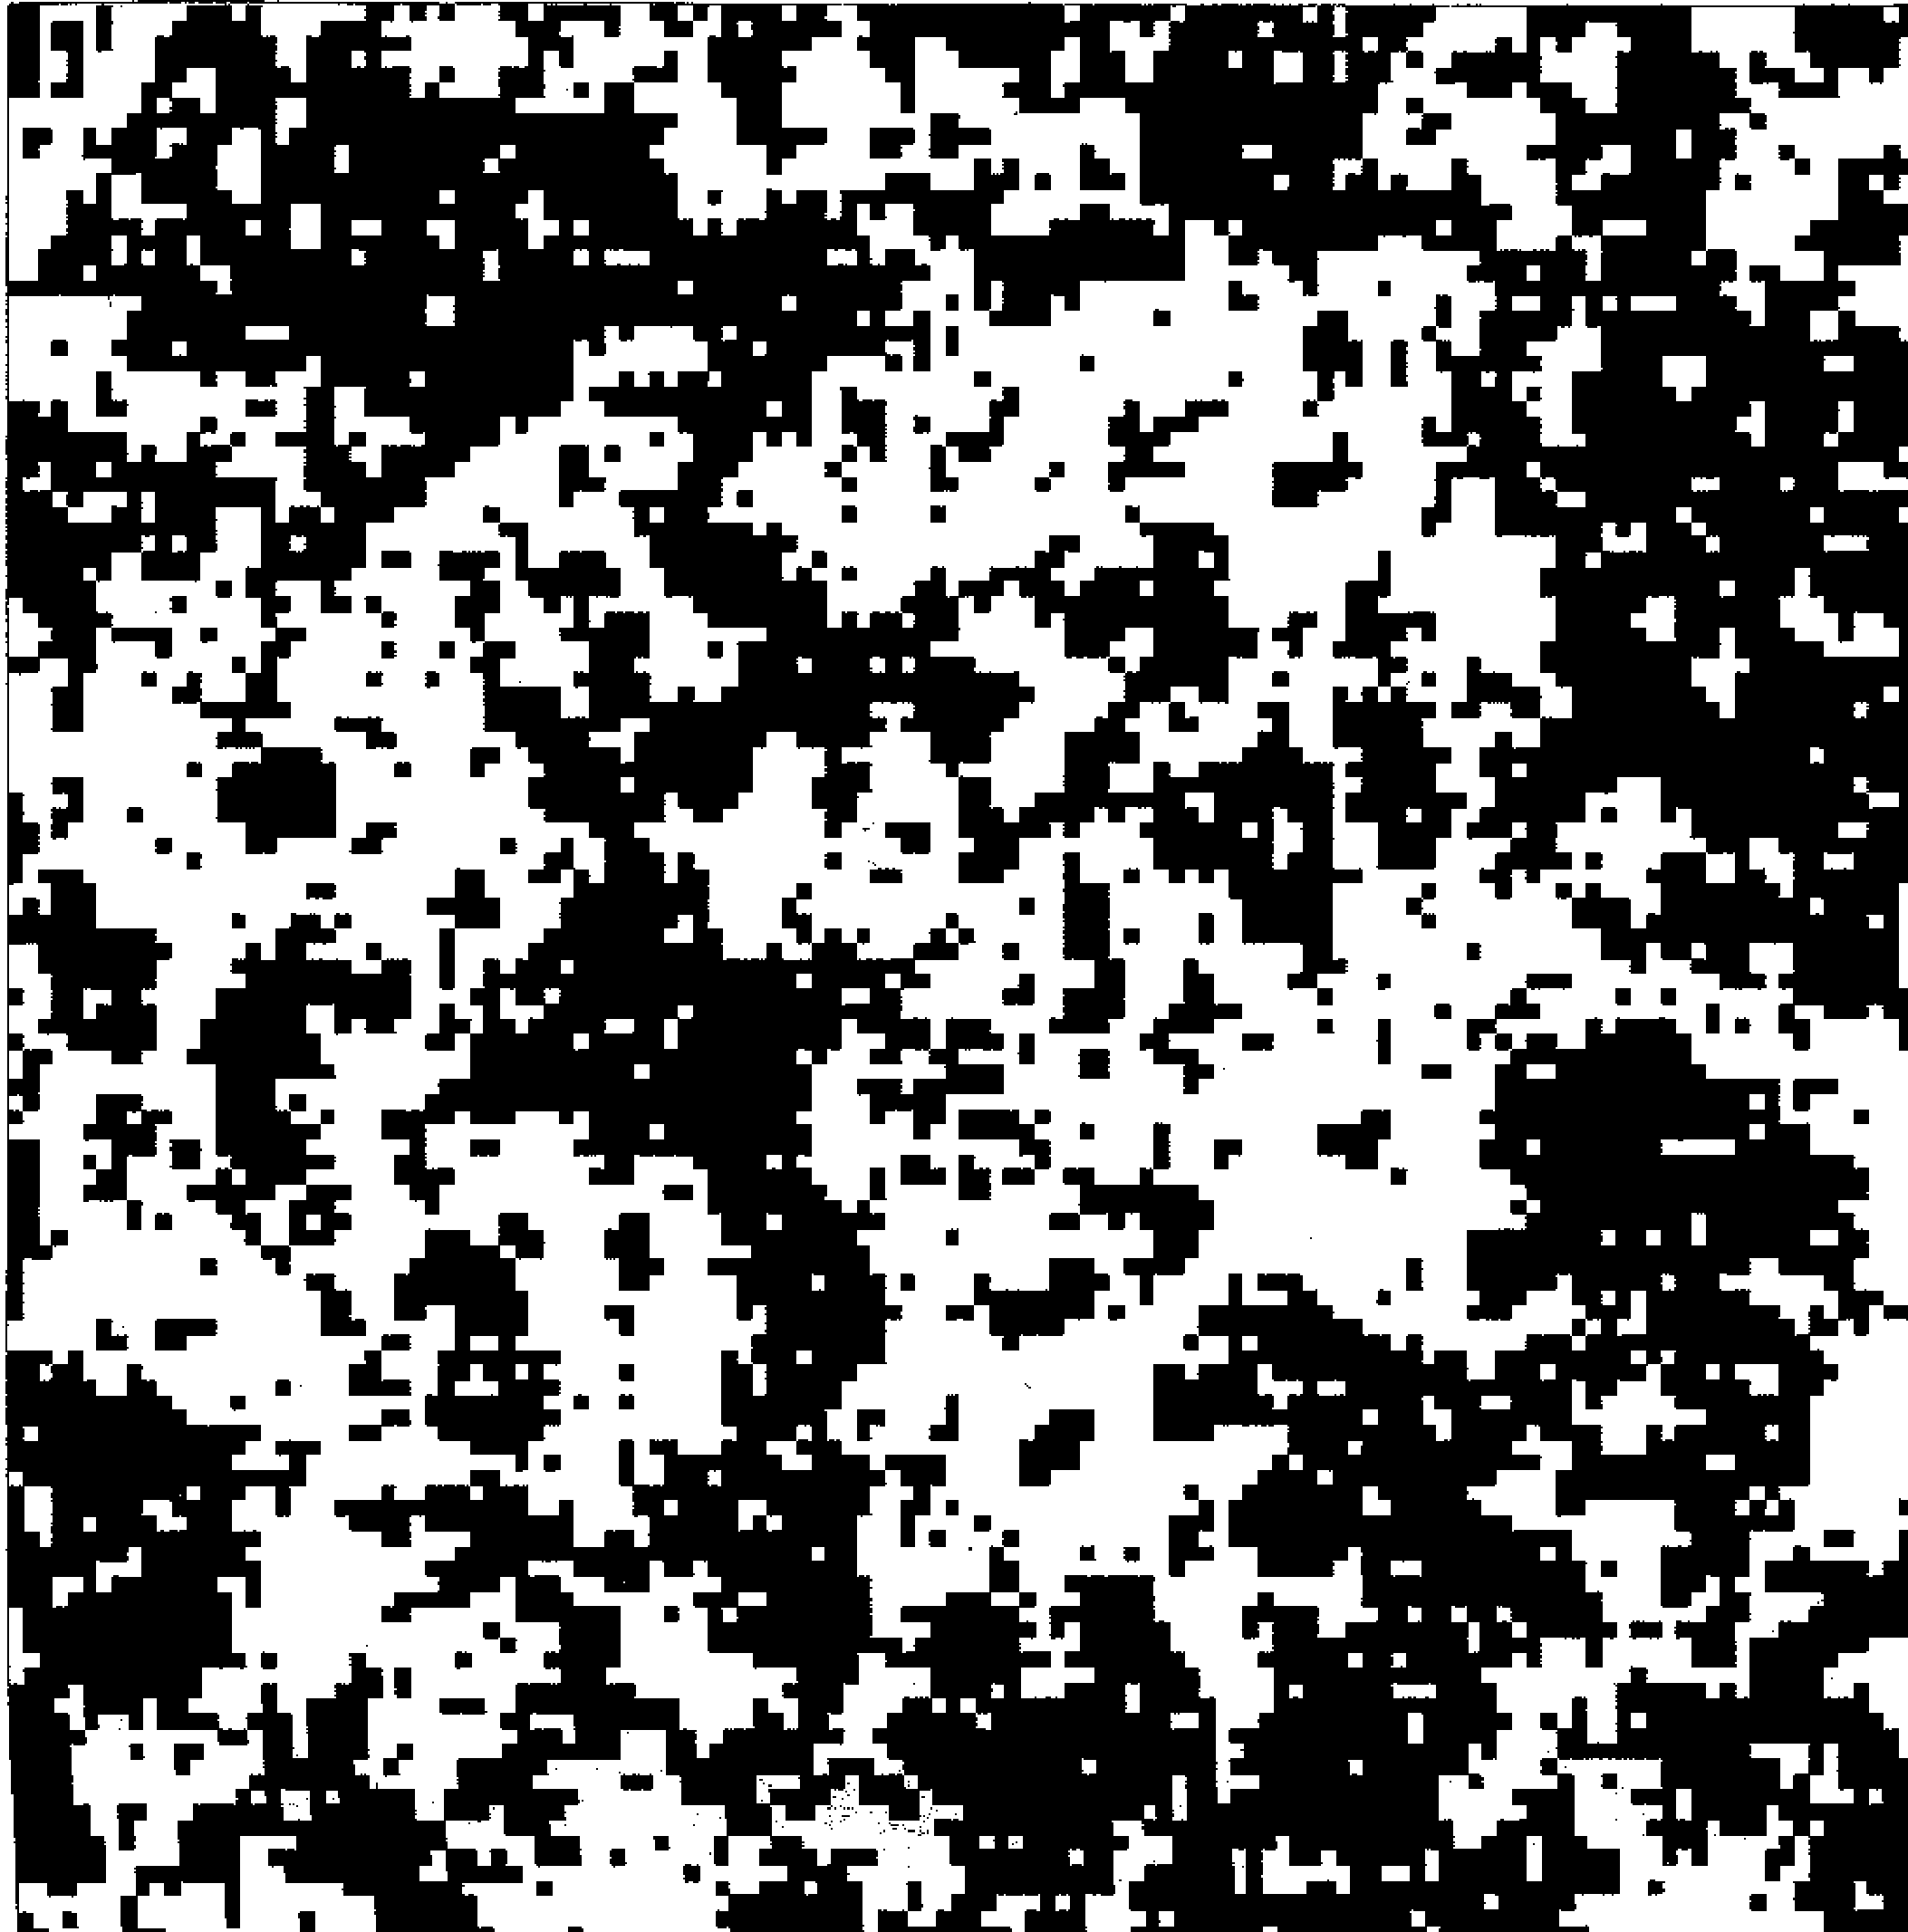
\includegraphics[width=7.5cm,clip=true]{Figs/supercrit}}
\vspace*{10mm}\centerline{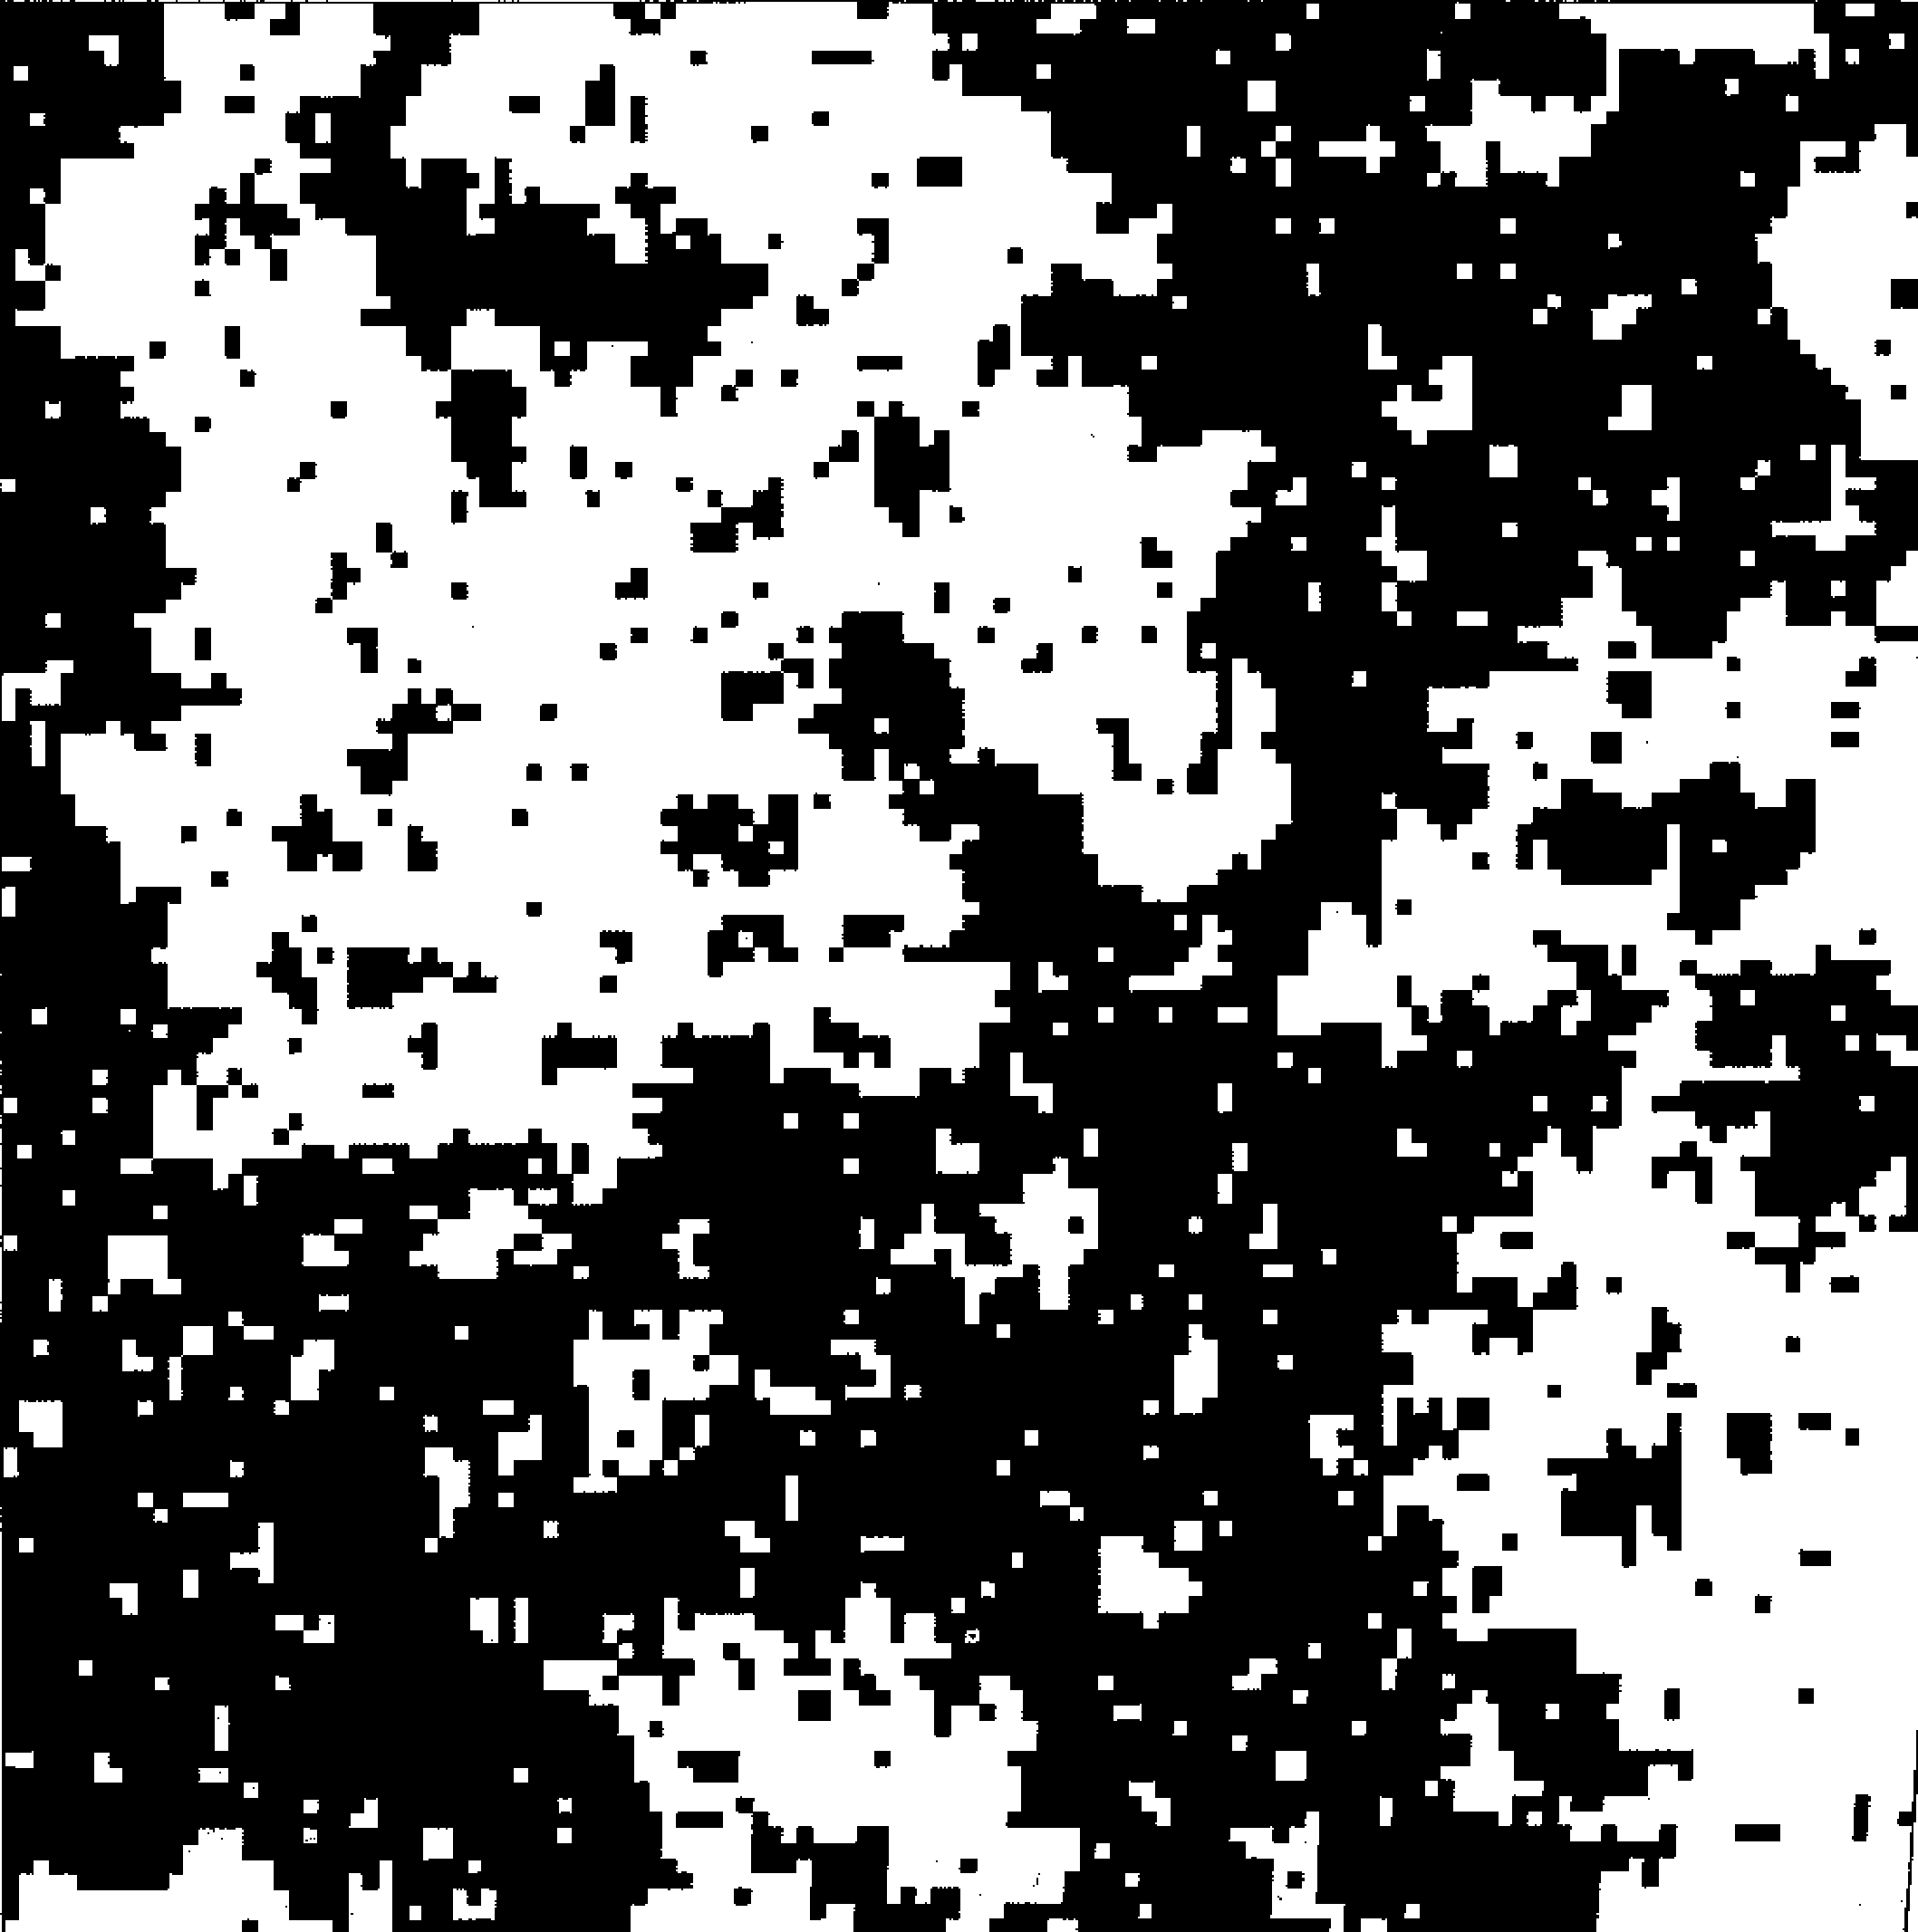
\includegraphics[width=7.5cm,clip=true]{Figs/crit}}
\vspace*{10mm}
\centerline{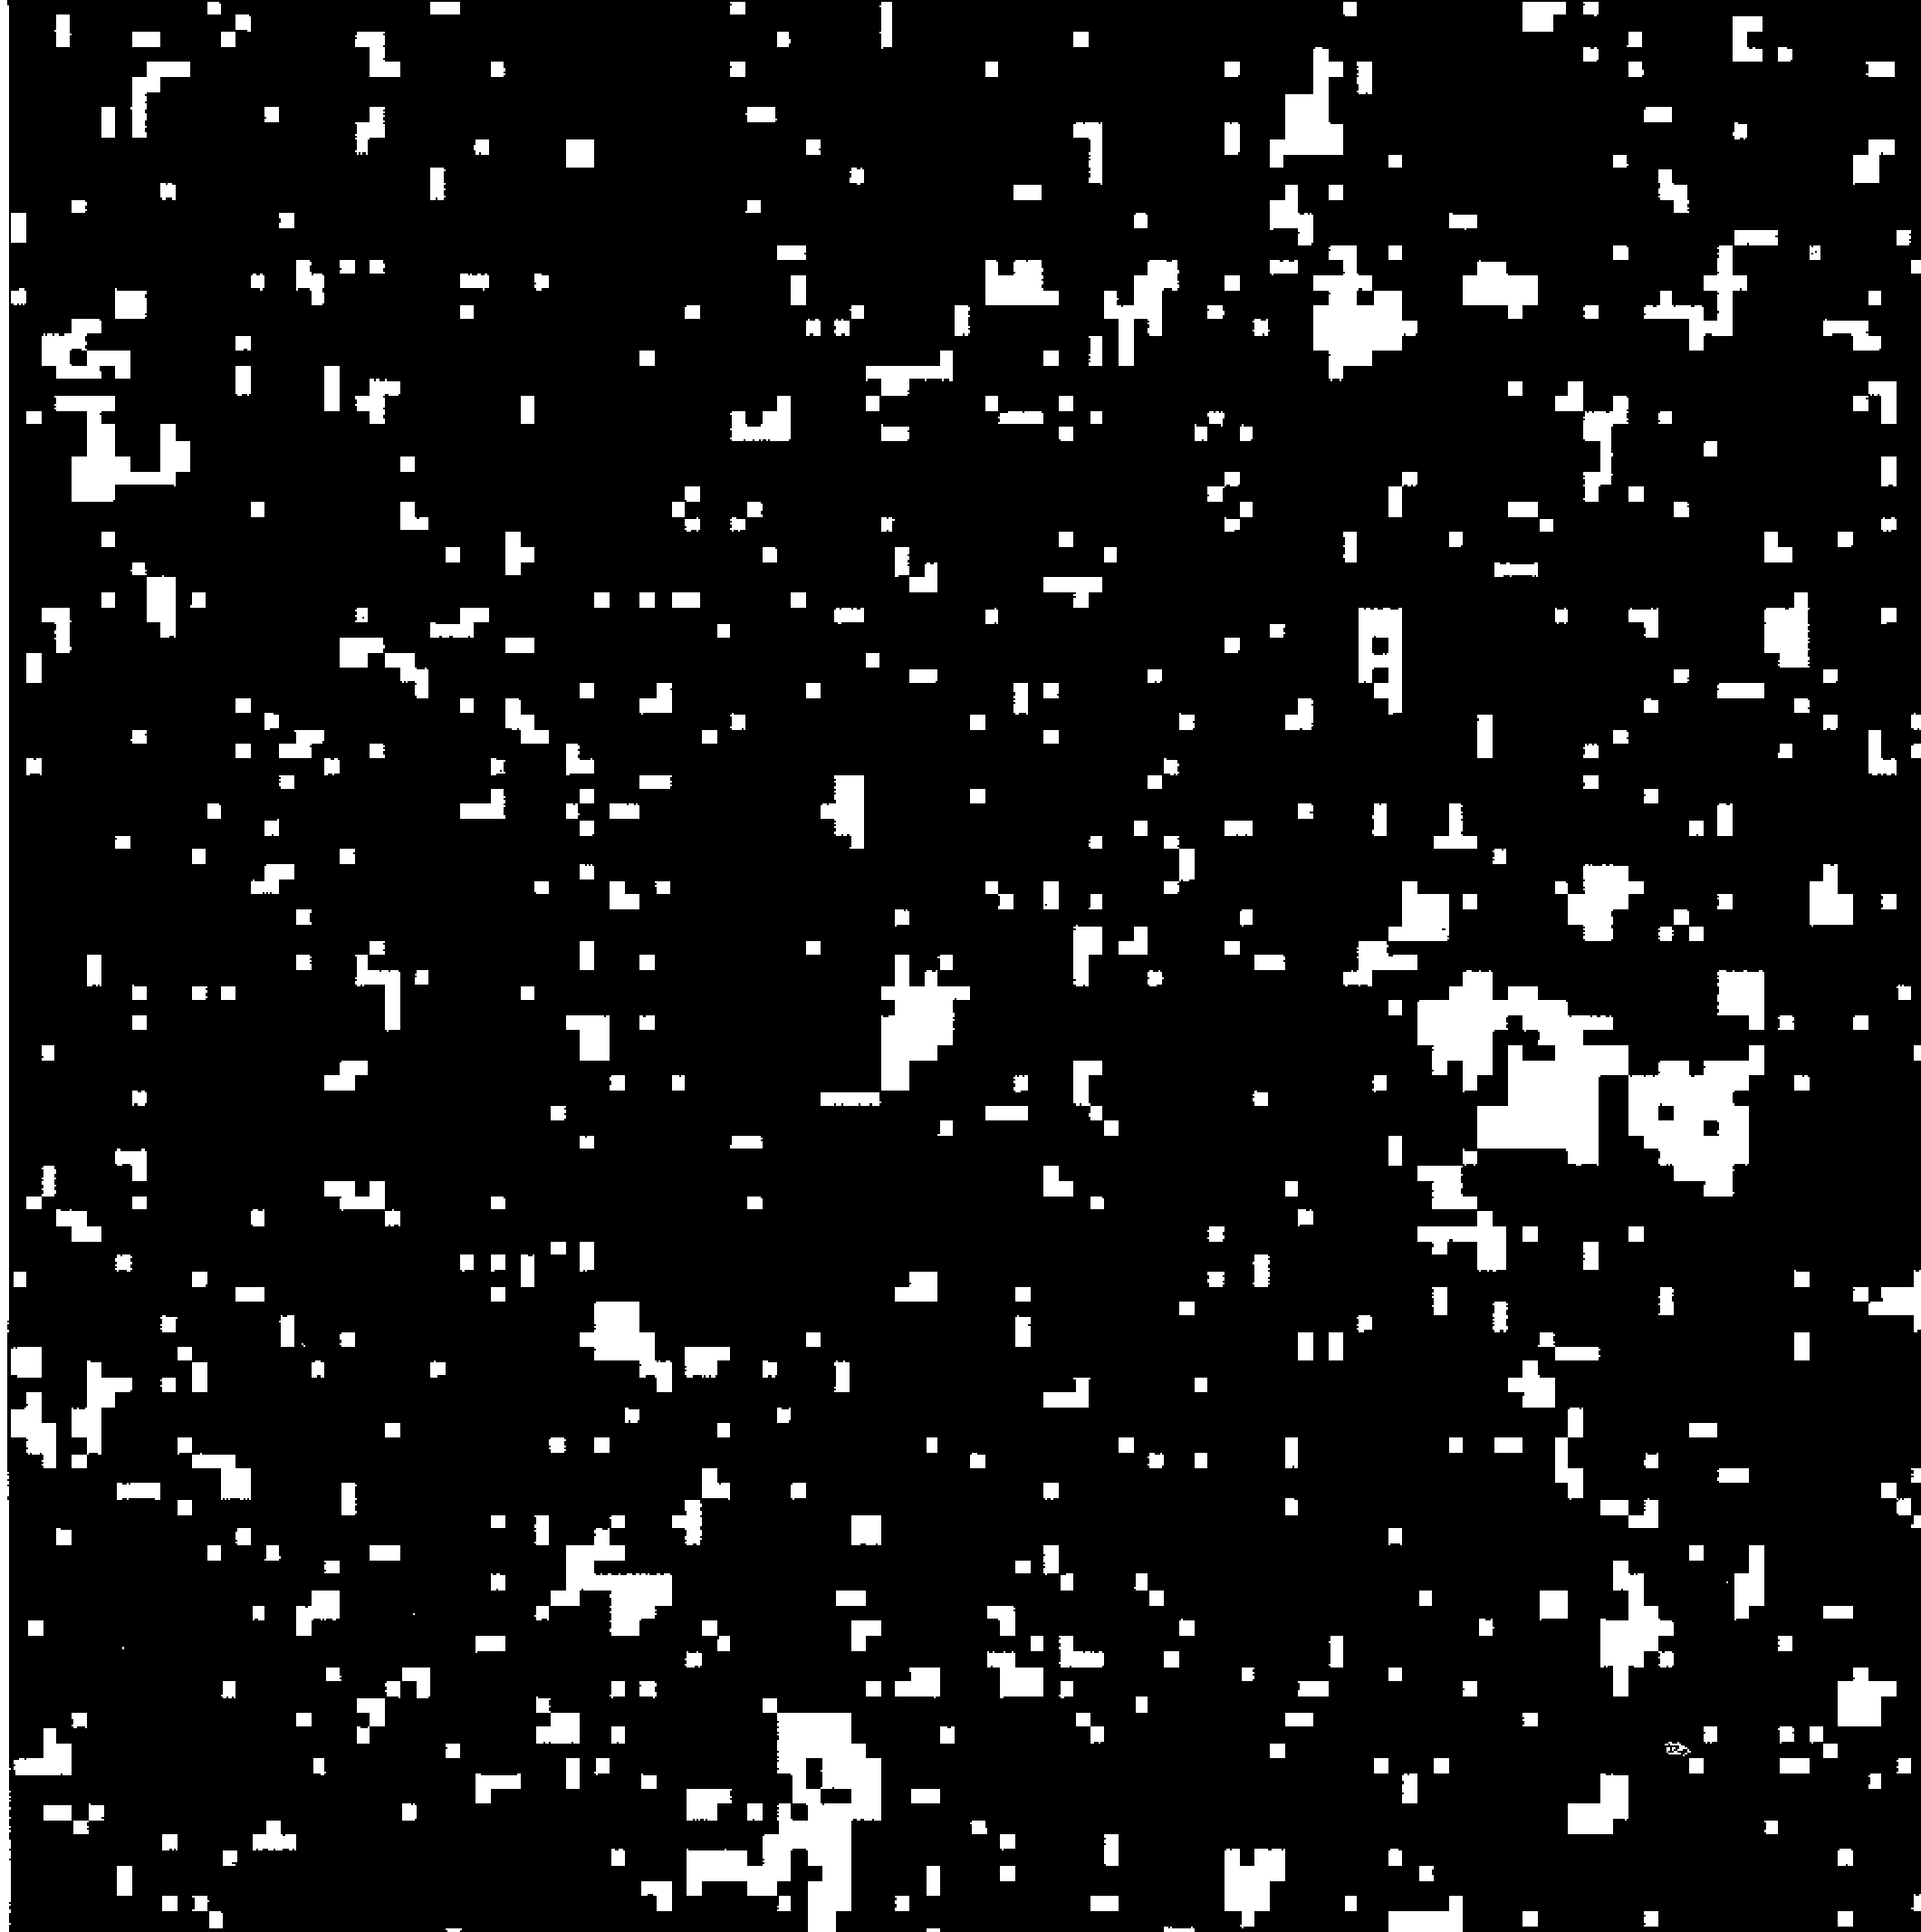
\includegraphics[width=7.5cm,clip=true]{Figs/subcrit}}
%}
\es
%%%%%%%%%%%%%%%%%%%%%%%%%%%%%%%%%%%%%%%%%%%%%%%%%%%%%%%%%%%%%%%%%%%%


%%%%%%%%%%%%%%%%%%%%%%%%%%%%%%%%%%%%%%%%%%%%%%%%%%%%%%%%%%%%%%%%%%%%%%
\bs
\bi

\item Despite its simplicity,  critical point universality
implies that critical exponents of Ising model are same as those of
real magnets.

\item Ising model therefore provides a simple, yet {\em quantitatively} accurate
representation of the critical properties of a whole range of real magnetic
(and indeed fluid) systems.

\item This universal feature of the model is largely
responsible for its ubiquity in the field of critical phenomena.

\ei
\es

%%%%%%%%%%%%%%%%%%%%%%%%%%%%%%%%%%%%%%%%%%%%%%%%%%%%%%%%%%%%%%%%%%%%%%


\bs
\slidetitle{\small Exact Solutions: the 1D Ising chain}

\bi

\item  Why is the 2D Ising model the simplest to exhibit a phase
transition? What happens in 1D?

\item In fact there is no phase transition in 1D for $T>0$.

\item Consider the ground state of a 1D Ising chain and a state with
various "domain walls" dividing spin-up and spin-down regions.

\item Transform from a spin representation to a domain wall
representation.

\ei
\es
%%%%%%%%%%%%%%%%%%%%%%%%%%%%%%%%%%%%%%%%%%%%%%%%%%%%%%%%%%%%%%%%%%%%%%%%%%%%
\bs\bi

\item Domain walls can occur on the bonds of the lattice of which there
are N-1. If a wall is present, the energy cost is $\Delta=2J$
independent of position (ie domain walls don't interact).

\item The partition function of system is

\[
Z=Z_1^{N-1}
\]

where for a single domain wall,

\[
Z_1=e^{\beta J} + e^{\beta (J-\Delta)}=e^{\beta J}(1+e^{-\beta\Delta})
\]

so

\[
\beta f\equiv \beta F/(N-1)=-\ln Z_1=-\beta J-\ln(1+e^{-\beta\Delta})
\]

\item The second term arises from the free energy of the domain wall population and since it is negative for all $T>0$, the free energy is
lowered by having domain walls, ie the system is always disordered.

\ei\es
%%%%%%%%%%%%%%%%%%%%%%%%%%%%%%%%%%%%%%%%%%%%%%%%%%%%%%%%%%%%%%%%%%%%%%%

\bs

\slidetitle{\small More general 1D spin systems}
\bi

\item For a 1-d assembly of $N$ spins each having $m$
discrete energy states, and in the presence of a magnetic field,
possible to get free energy via the transfer matrix method.
Let us start by assuming that the assembly has cyclic boundary conditions, then the
total energy of configuration $\{s\}$ is

\ei
{\small
\begin{eqnarray*}
H(\{s\})&=&-\sum_{i=1}^N (Js_is_{i+1}+Hs_i)\\
\:&=&-\sum_{i=1}^N (Js_is_{i+1}+H(s_i+s_{i+1})/2)\\
\:&=&\sum_{i=1}^N E(s_i,s_{i+1})
\end{eqnarray*}
where we have defined $E(s_i,s_{i+1})=-Js_is_{i+1}-H(s_i+s_{i+1})/2$.
}

\es

\bs
Now the partition function may be written

{\small
\begin{eqnarray}
\label{eq:tm}
Z_N &=& \sum_{\{s\}}\exp\left(-\beta H(\{s\})\right)\nonumber \\
 &=&\sum_{\{s\}}\exp\left(-\beta[E(s_1,s_2)+E(s_2,s_3)+....E(s_N,s_1)]\right) \nonumber\\
 &=&\sum_{\{s\}}\exp\left(-\beta E(s_1,s_2)\right)\exp\left(-\beta E(s_2,s_3)\right)....\exp\left(-\beta E(s_N,s_1)\right) \nonumber\\
&=&\sum_{i,j,...,l=1}^m V_{ij}V_{jk}...V_{li} \label{eq:Vs}
\end{eqnarray}}
where the $V_{ij}=\exp(-\beta E_{ij})$ are elements of an $m \times m$
matrix ${\bf V}$, known as the transfer matrix.

\begin{itemize}

\item Transpires that the sum over the matrix elements in equation~(\ref{eq:Vs})
is simply just the trace of ${\bf V}^N$, given by the sum of its eigenvalues:-

\[
Z_N=\lambda_1^N+\lambda_2^N+...\lambda_m^N 
\]

\ei\es

%%%%%%%%%%%%%%%%%%%%%%%%%%%%%%%%%%%%%%%%%%%%%%%%%%%%%%%%%%%%%%%%%%%%%%%%%%

\bs\bi

\item As $N\to \infty$, largest eigenvalue $\lambda_1$ dominates since 
$(\lambda_2/\lambda_1)^N$ vanishes. Consequently  $Z_N=\lambda_1^N$

\item Specializing to the case of the simple Ising model in the presence of
an applied field $H$, the transfer matrix takes the form 

\[
{\bf V}(H)=\left(
\begin{array}{cc}
e^{\beta(J+H)} & e^{-\beta J} \\
e^{-\beta J}   & e^{\beta(J-H)}
\end{array} \right)
\]

\item This matrix has two eigenvalues which can be readily calculated in the
usual fashion. They are

\[
\lambda_{\pm}=e^{\beta J}\cosh(\beta H) \pm \sqrt{e^{2\beta J}\sinh^2\beta H+e^{-2\beta J}}.
\]

Hence the free energy per spin $f=-k_BT\ln \lambda_+$ is
\ei

\[
f=-k_BT\ln \left[e^{\beta J}\cosh(\beta H) + \sqrt{e^{2\beta J}\sinh^2\beta H+e^{-2\beta J}}\right].
\]

\es

%%%%%%%%%%%%%%%%%%%%%%%%%%%%%%%%%%%%%%%%%%%%%%%%%%%%%%%%%%%%%%%%%%%%%%%%%
%%%%%%%%%%%%%%%%%%%%%%%%%%%%%%%%%%%%%%%%%%%%%%%%%%%%%%%%%%%%%%%%%%%%%%
\bs
\slidetitle{Mean field theory}
\bi

\item The critical behaviour of most model systems cannot be found
analytically.

\item A few exceptions eg. 2D Ising model (but not the 3D) have
been solved ($\beta=\frac{1}{8}, \nu=1, \gamma=\frac{7}{4}$.
$T_c=-2J/\ln(\sqrt{2}-1)\approx 2.269J$)

\item But such solutions provide little insight into the essential nature
of criticality.

\item When an exact solution is elusive, can try to make simplifying
assumptions to calculate critical behaviour. Mean field theory is such
an approximation scheme.


\ei
\es


%%%%%%%%%%%%%%%%%%%%%%%%%%%%%%%%%%%%%%%%%%%%%%%%%%%%%%%%%%%%%%%%%%%%%%%%%%%%
\bs

\slidetitle{\small Mean field theory}

\bi

\item Look for a mean field expression for the free energy of the Ising model. Write

\[
s_i=\langle s_i\rangle+(s_i-\langle s_i\rangle)=m+(s_i-m)=m+\delta s_i
\]

Then 
\begin{small}
\begin{eqnarray*}
{\cal H}_I&=&-J\sum_{<i,j>}[m+(s_i-m)][m+(s_j-m)]-H\sum_i s_i\nonumber\\
&=&-J\sum_{<i,j>}[m^2+m(s_i-m)+m(s_j-m)+\delta s_i\delta s_j]-H\sum_i s_i\nonumber\\
&=&-J\sum_{i}(qms_i-qm^2/2)-H\sum_i s_i-J\sum_{<i,j>}\delta s_i\delta s_j
\end{eqnarray*}
\end{small}
where the sum $\sum_{<i,j>}$ over bonds of a quantity which independent of $s_j$, is just $q/2$ times that quantity.  

\item Now the mean field approximation is to ignore the last term giving

\[
{\cal H}_{mf}=-\sum_{i}H_{mf}s_i+NqJm^2/2
\]
with $H_{mf}\equiv Jqm+ H$. 
\ei\es

\bs\bi


\item It follows that the partition function is

\[
Z=e^{-\beta qJm^2N/2}[2\cosh(\beta(qJm+H))]^N
\]

\item so the free energy is

\[
F(m)=NJqm^2/2-Nk_BT\ln[2\cosh(\beta (qJm+H)]\:.
\]

\item From which the magnetisation follows as

\[
m=-\frac{1}{N}\frac{\partial F}{\partial H}=\tanh(\beta(qJm+H))
\]

\item To find $m(H,T)$, we must numerically solve this last equation self consistently. 


\ei\es
%%%%%%%%%%%%%%%%%%%%%%%%%%%%%%%%%%%%%%%%
\bs
\slidetitle{\small Spontaneous symmetry breaking}
\bi

\item Mean field method reveals what is happening in the Ising model near
the critical temperature $T_c$. 

\item Plot $\beta F(m)/N$ vs $T$ for $H=0$:



\vspace*{8cm}

\item For $H=0$, $F(m)$ is symmetric in $m$. At high $T$,  entropy dominates $\to$
single minimum in $F(m)$ at $m=0$. 

\item As $T$ is lowered, there comes a
point ($T=T_c$) where the curvature of $F(m)$ at the origin changes
sign; ie.

\[
\frac{\partial^2 F}{\partial m^2}=0.
\]

\ei\es
%%%%%%%%%%%%%%%%%%%%%%%%%%%%%%%%%%%%%%%%%%%%%%%%%%%%%%%%%%%%%%%%%%%%%%
\bs\bi

\item At lower temperature: two minima at nonzero
$m=\pm m^\star$, where the {\em equilibrium magnetisation}
 $m^\star$ is the positive root (calculate explicitly below) of 

\begin{equation}
m^\star=\tanh(\beta Jqm^\star)= \tanh(\frac{m^\star T_c}{T}) 
\end{equation}

\item $m^\star=0$ which remains a root of this equation, is clearly an
unstable point for $T<T_c$ (since $F$ has a maximum there).

\item Example of spontaneous symmetry breaking: Pair of ferromagnetic states (spins mostly up, or spins mostly
down) which -- by symmetry-- have the same free energy, lower than the
unmagnetized state.

\ei\es
%%%%%%%%%%%%%%%%%%%%%%%%%%%%%%%%%%%%%%%%%%%%%%%%%%%%%%%%%%%%%%%%%%%%%

\bs

\slidetitle{\small Phase diagram}

\bi

\item The resulting zero-field magnetisation curve:
like:
\vspace*{8cm}

\item Sudden change of behaviour at $T_c$ (continuous phase transition).

\item For $T<T_c$, arbitrary which of the two roots $\pm m^\star$ is
chosen; typically it will be different in different parts of the sample
(giving macroscopic ``magnetic domains''). 
\ei\es

%%%%%%%%%%%%%%%%%%%%%%%%%%%%%%%%%%%%%%%%%%%%%%%%%%%%%%%%%%%%%%%%%%%%%

\bs\bi

\item Picture is {\em qualitatively modified} by a field $H$
$\to$ always a  magnetization, even  $T\gg T_c$ (no
phase transition).

\vspace*{10cm}

\item Sit below $T_c$ with $H>0$ and gradually reduce $H$ so that it
becomes negative. $\Rightarrow$ {\em very} sudden change of behaviour
at $h=0$: the equilibrium state jumps discontinuously from $m=m^\star$
to $m=-m^\star$. 

\item This is called a first order phase transition.  

\ei\es

%%%%%%%%%%%%%%%%%%%%%%%%%%%%%%%%%%%%%%%%%%%%%%%%%%%%%%%%%%%%%%%5

\bs


{\em First order transition:} magnetisation (or similar order parameter)
depends discontinuously on other variable (such as $h$ or $T$).

{\em Continuous transition:} Change of functional form, but no
discontinuity in $m$; typically, however, $(\partial m/\partial T)_h$
(or similar) is either discontinuous, or diverges.

\bi
\item Say that the phase diagram of the magnet in
the $H,T$ plane shows a line of first order phase transitions,
terminating at a continuous transition, which is the critical point.
\ei
\es
%%%%%%%%%%%%%%%%%%%%%%%%%%%%%%%%%%%%%%%%%%%%%%%%%%%%%%%%%%%%%%%%%%%%%%%
\bs





\bs
Mean field predictions for critical exponents:\\
{\bf Zero H solution}
\vspace*{5mm}
\[
m=\tanh(\frac{mT_c}{T}) 
\]

\bi 

\item We look for a solution where $m$ is small ($\ll 1$). Taylor expanding the tanh
function  yields

\[
m=\frac{mT_c}{T}-\frac{1}{3}\left(\frac{mT_c}{T} \right)^3 +O(m^5)
\]

\item Then $m=0$ is one solution. The other solution is given by

\[
m^2=3\left(\frac{T}{T_c} \right)^3\left(\frac{T_c}{T} -1\right)
\]

\item Now, for $T$ close to $T_c$ (i.e. small $m$), and
writing $t=(T-T_c)/T_c$, one finds

\[
m^2\simeq -3t
\]

i.e.
\begin{eqnarray*}
m=& 0           &    {\rm for} \hspace*{3mm} T>T_c  \\
m=& \pm\sqrt{-3t} & {\rm for}   \hspace*{3mm} T<T_c 
\end{eqnarray*}

\ei
\es

%%%%%%%%%%%%%%%%%%%%%%%%%%%%%%%%%%%%%%%%%%%%%%%%%%%%%%%%%%%%%%%%%%%%%%

\bs

{\bf Finite (but small) field solution}
\bi

\item In a small field we can make the Taylor expansion

\[
m=\frac{mT_c}{T}-\frac{1}{3}\left(\frac{mT_c}{T} \right)^3 +\frac{H}{kT}
\]

\item Consider now the isothermal susceptibility 

\begin{eqnarray*}
\chi & \equiv & \left(\frac{\partial m}{\partial H}\right)_T\\
     & =     & \frac{T_c}{T}\chi - \left(\frac{T_c}{T}\right)^3 \chi m^2 + \frac{1}{k_BT}  
\end{eqnarray*}

\item Then 

\[
\chi \left[ 1-\frac{T_c}{T} +\left(\frac{T_c}{T}\right)^3 m^2  \right]=\frac{1}{k_bT}
\]


\ei
\es

%%%%%%%%%%%%%%%%%%%%%%%%%%%%%%%%%%%%%%%%%%%%%%%%%%%%%%%%%%%%%%%%%%%%%%

\bs
\bi

\item Hence near $T_c$

\[
\chi=\frac{1}{k_BT_c}\left(\frac{1}{t+m^2}\right)
\]

Then
\begin{eqnarray*}
\chi=& (k_BT_ct)^{-1} & {\rm for} \hspace*{3mm} T> T_c \\
\chi=& (-2k_BT_ct)^{-1} & {\rm for}   \hspace*{3mm}T \le T_c 
\end{eqnarray*}
where one has to take the non-zero value for $m$ below $T_c$ to ensure
+ve $\chi$, i.e. thermodynamic stability.

\vspace*{10cm}

\ei
\es


%%%%%%%%%%%%%%%%%%%%%%%%%%%%%%%%%%%%%%%%%%%%%%%%%%%%%%%%%%%%%%%%%%%%%%

\bs
\slidetitle{\small Landau theory}
\bi

\item Landau theory is more general type of mean field theory. Not
based on a particular microscopic model. 

\item Starting point is the Helmholtz free energy, which  is written as
a truncated power series expansion of the order parameter. 

\item For a ferromagnet (up-down spin symmetry) this takes the form

\[
F(m)=F_0+a_2m^2+a_4m^4
\]

\item Equilibrium $m$ is that for which $F(m)$ is minimum.

\item Plots of the Landau free energy (for various $a_2$, with $a_4>0$ show how it gives rise to 
a critical point


\ei\es

%%%%%%%%%%%%%%%%%%%%%%%%%%%%%%%%%%%%%%%%%%%%%%%%%%%%%%%%%%%%%%%%%%%%%%%%%

\bs

\centerline{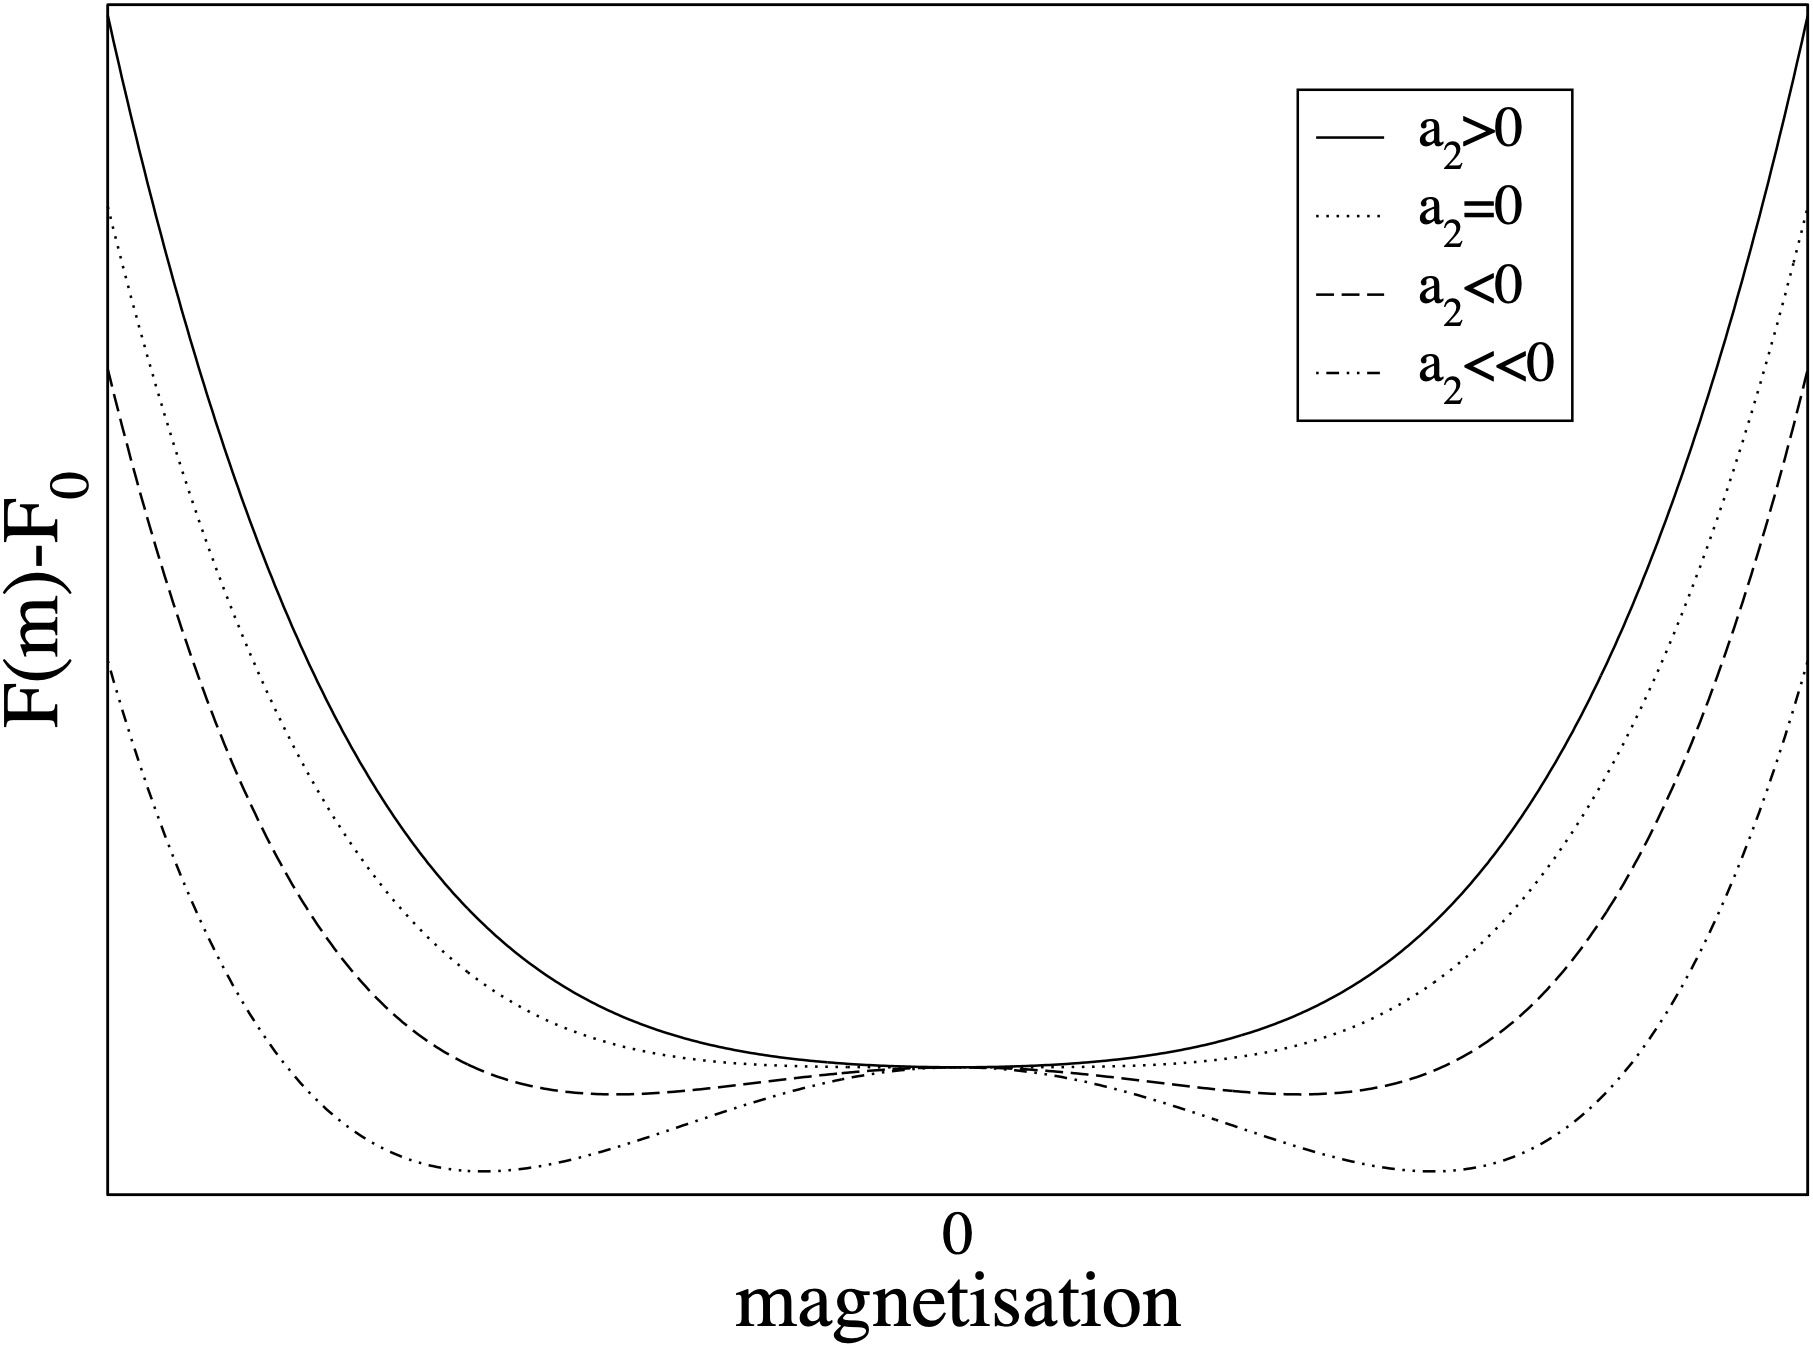
\includegraphics[width=10.3cm,clip=true]{Figs/landau}}

\bi

\item Thermodynamics tells us that the system adopts the state of lowest
free energy.

\item  Thus for $a_2>0$, the system will have $m=0$, i.e. will be in the disordered (or
paramagnetic) phase.


\item For $a_2<0$, minimum of $F$ occurs at a two symmetric minima at
$m=\pm m_0$  i.e., the ordered phase is the stable one.

\ei\es
%%%%%%%%%%%%%%%%%%%%%%%%%%%%%%%%%%%%%%%%%%%%%%%%%%%%%%%%%%%%%%%%%%%%%%%%

\bs
\bi

\item $a_2=0$ corresponds to the critical point which marks
the border between the ordered and disordered phases. 

\item Thus clearly $a_2$ controls the deviation from the critical
temperature, i.e.

\[
a_2=\tilde{a_2} t
\]
where $t$ is the reduced temperature.

\item Can now attempt to calculate critical exponents. First find
equilibrium magnetisation, corresponding to the minimum of the Landau free
energy:

\[
\frac{dF}{dm}=2\tilde{a_2} tm+4a_4m^3=0
\]

i.e.
\[
m\propto (-t)^{1/2},
\]
so $\beta=1/2$, (mean field result).

\ei\es
%%%%%%%%%%%%%%%%%%%%%%%%%%%%%%%%%%%%%%%%%%%%%%%%%%%%%%%%%%%%%%%%%%%%%%%%%
\bs
\bi

\item We can calculate the effect of a small field $H$ if we sit at the
critical temperature $T_c$. Since $a_2=0$, we have

\[
F(m)=F_0+a_4m^4-Hm
\]

\[
\frac{\partial F}{\partial m}=0 \Rightarrow m(H,T_c)=\left(\frac{H}{4a_4}\right)^{1/3}
\]

or

\[
H \sim m^\delta \hspace*{1.5cm} \delta=3
\]
which defines a second critical exponent. 

\item Thirdly, Magnetic susceptibility at zero field

\[
\chi=\left(\frac{\partial m}{\partial H}\right)_{T,V} \sim |T-T_c|^{-\gamma}
\]

{\em Exercise}: Show that $\gamma=1$.

\item Finally heat capacity (per site or per unit volume) $C_H$, for $H=0$:

\[
C_H \sim |T-T_c|^{-\alpha}
\]
with $\alpha=0$.

\ei
\es

%%%%%%%%%%%%%%%%%%%%%%%%%%%%%%%%%%%%%%%%%%%%%%%%%%%%%%%%%%%%%%%%%%%%%%

\bs
\bi

\item In real ferromagnets, as well as in more sophisticated theories, the
exponents $\beta$ and $\gamma$ are not the simple fraction and integers
found here.


\item This failure of mean field theory to predict the correct
exponents is of course traceable to their neglect of correlations.

\ei
\es
{\tiny
%\begin{table}[h]
\begin{center}
\begin{tabular}{|c|c|c|c|c|}\hline
$\:$ & {\rm Mean Field} & $d=1$ & $d=2$ & $d=3$ \\
{\rm Critical temperature} $k_BT/qJ$  & $1$ & $0$ & $0.5673$ & $0.75$ \\
{\rm Order parameter exponent} $\beta$ & $\frac{1}{2}$ &- & $\frac{1}{8}$ &
$0.325 \pm 0.001$ \\
{\rm Susceptibility exponent} $\gamma$ &  $1$ & $\infty$ & $\frac{7}{4}$ & $1.24 \pm 0.001$ \\
{\rm Correlation length exponent} $\nu$ & $\frac{1}{2}$ & $\infty$ & $1$ &
$0.63\pm 0.001$ \\ \hline
\end{tabular}
\label{tab:exponents}
%\caption{Comparison of true Ising critical exponents with their mean
%field theory predictions in a number of dimensions.}
\end{center}
%\end{table}
}



%%%%%%%%%%%%%%%%%%%%%%%%%%%%%%%%%%%%%%%%%%%%%%%%%%%%%%%%%%%%%%%%%%


\bs
\slidetitle{\small Lattice Gas model}

\bi 

\item A crude representation of a fluid.

\item Particles can occupy the sites of a hypercubic lattice.

\item Occupancy variables $c_i=1$ (occupied) or $c_i=0$ (vacant). 

\item The average particle number density is given $c=L^{-d}\sum_ic_i$

\item Hamiltonian:

\[
{\cal H}_{LG}=-\epsilon\sum_{<i,j>}c_ic_j -\mu\sum_ic_i
\]

\item Particle density fluctuates around a mean value controlled by $\mu$. 

\ei
\es
%%%%%%%%%%%%%%%%%%%%%%%%%%%%%%%%%%%%%%%%%%%%%%%%%%%%%%%%%%%%%%%%%

\bs
\bi

\item The lattice gas model maps onto (is {\em isomorphic} to) the Ising model, extending its
applicability to fluids. 

\item Write the partition function of the lattice gas:

\[
\Xi=\sum_{\{c\}}\exp\left[\beta \epsilon\sum_{<i,j>}c_ic_j +\beta\mu\sum_ic_i\right]
\]

\item Now change variables to 

\[
c_i=(1+s_i)/2; \hspace*{1cm} J=\frac{\epsilon}{4}\hspace*{1cm}
h=\frac{\epsilon q+2\mu}{4}
\]
Hence 

\[
{\cal H}_{LG}={\cal H}_{\rm I} + {\rm constant}
\]

\item Since the last term does not depend on the configuration, it has no physical implications.

\ei
\es
%%%%%%%%%%%%%%%%%%%%%%%%%%%%%%%%%%%%%%%%%%%%%%%%%%%%%%%%%%%%%%%%%%%%%%%%%%%%%%



\bs\bi

\item {\bf Phase diagram} Using the translation rules we can plot the phase diagram of the
lattice gas in the $\mu-T$ plane.

\vspace*{8cm}

\item Again there is a line of first order phase transitions terminating at a
critical point. 

\item First order line means that if $T<T_c$ we smoothly
increase the chemical potential through coexistence,
density of particles $c$ jumps discontinuously:

\[
c_{\rm gas}=\frac{1-m^\star}{2} \to c_{\rm liquid}=\frac{1+m^\star}{2}
\]
These values merge at $T_c$, the gas-liquid critical point. At higher
temperatures, the distinction between the phases disappears.

\item {\bf Real Fluids}. Compare this with a real fluid. Main
difference is that the lattice gas has ``Particle-hole'' symmetry,
$c\to 1-c$. $\Rightarrow$ Phase diagram in a real fluid looks lopsided.

\ei\es


%%%%%%%%%%%%%%%%%%%%%%%%%%%%%%%%%%%%%%%%%%%%%%%%%%%%%%%%%%%%%%%%%%%%%%%%%
\bs
\slidetitle{\small Series expansion}

\bi
\item Perturbation theory, going beyond mean field approximation. 

\item Seeks to deduce results for the critical
region using known results obtained away from criticality.

\item Simple example is the high-T series, which expresses 
Boltzmann factor as expansion in $1/T$ (assumed small). 

\[
\exp(-{\cal H}/k_BT)=1-{\cal H}/k_BT +\frac{1}{2!}({\cal H}/k_BT)^2+.....
\]

\item Successively higher terms characterise
correlations over successively larger distances.

\item  Known results for the high-T fully disordered phase permit the
calculation of $Z$ using the significant terms in this expansion. 

\item Method breaks down close to $T_c$, due to divergent correlation
length.

\ei
\es
%%%%%%%%%%%%%%%%%%%%%%%%%%%%%%%%%%%%%%%%%%%%%%%%%%%%%%%%%%%%%%%%%%%%
\slidetitle{\small The Static Scaling Hypothesis}

\bi

\item The static scaling hypothesis provides a basis for power law
behaviour. Moreover it predicts the existence of so-called {\em scaling
phenomena} in near-critical systems.

\item The hypothesis asserts that: near criticality, the free energy is
a so-called {\em generalised homogeneous functions} of the
thermodynamic fields.

\item A function of two variables $g(u,v)$ is called a generalised homogeneous
function if it has the property

\[
g(\lambda^au,\lambda^bv)=\lambda g(u,v)
\]
{\bf for all $\lambda$}, where the parameters a and b (known as scaling parameters)
are constants.  


\item For such functions one can always implement a {\em change of scale},
to reduce the dependence on two variables (e.g. $t$ and $h$)
to dependence on one new variable.  
\ei\es
%%%%%%%%%%%%%%%%%%%%%%%%%%%%%%%%%%%%%%%%%%%%%%%%%%%%%%%%%%%%%%%%%%%%%%%

\bs\bi

\item The arbitrary scale factor $\lambda$ can be chosen as
$\lambda^a=u^{-1}$ giving

\[
g(u,v)=u^{1/a}g(1,\frac{v}{u^{b/a}})
\]

\item Thus $g(u,v)$  satisfies a simple power law in $\it{one}$ variable, provided $v/u^{b/a}=C$. Note, however, that
this relationship specifies neither the function $g$ nor the parameters $a$ and $b$. 

\item Scaling hypothesis asserts that in the critical region,
the free energy $F$ is a generalised homogeneous function of 
thermodynamic fields

\item Thus for the ferromagnet (fields $t$ and $h$):

\[
F(\lambda^a t,\lambda^b h)=\lambda F(t,h) 
\]
\ei\es
%%%%%%%%%%%%%%%%%%%%%%%%%%%%%%%%%%%%%%%%%%%%%%%%%%%%%%%%%%%%%%%%%%%%%%%

\bs\bi


\item Without loss of generality, we can set $\lambda^a=t^{-1}$, implying
$\lambda=t^{-1/a}$ and $\lambda^b=t^{-b/a}$. 

Then
\[
F(t,h)=t^{1/a}F(1,t^{-b/a}h)
\]
where our choice of $\lambda$ ensures that the rhs is now a function of
a single variable $t^{-b/a}h$.

\item An expression for the magnetisation can be obtained simply by
taking the field derivative of $F$ 

\[
m(t,h)=-t^{(1-b)/a}m(1,t^{-b/a}h)
\]

In zero applied field $h=0$, this reduces to 
                   
\[
m(t,0)=(-t)^{(1-b)/a}m(1,0)
\]
where the r.h.s. is a power law in $t$.

\item Can now identify the exponent $\beta$ in terms of the scaling parameters $a$ and $b$.

\[
\beta=\frac{1-b}{a}
\]

\ei\es
%%%%%%%%%%%%%%%%%%%%%%%%%%%%%%%%%%%%%%%%%%%%%%%%%%%%%%%%%%%%%%%%

\bs
\bi


\item By differentiating the free energy, other
relations between scaling parameters and critical exponents may be
deduced. 

\item Such calculations yield the results  $\delta =
b/(1-b)$,$\gamma = (2b-1)/a$, and $ \alpha =(2a-1)/a$. Try it as an
exercise!

\item Relationships
between the critical exponents follow by
eliminating the scaling parameters from these equations. 

\item The principal results (known as ``scaling laws'') are:-

\begin{eqnarray*}
\alpha+\beta(\delta+1)=2 \\
\alpha+2\beta+\gamma=2
\end{eqnarray*}

\item Thus only two critical exponents need be specified, for all
others to be deduced. 

\ei\es 

%%%%%%%%%%%%%%%%%%%%%%%%%%%%%%%%%%%%%%%%%%%%%%%%%%%%%%%%%%%%%%%%%%%%%%%%%%%
\bs
\slidetitle{\small Experimental Verification of Scaling}

\bi
\item Experiments confirm the scaling hypothesis.

\item Rewriting the above expression for $m(t,h)$ in terms 
the exponents $\beta$ and $\delta$, one finds

\[
\frac{m(t,h)}{t^{\beta}}=m(1,\frac{h}{t^{\beta\delta}})
\]
where the RHS is a function of the single
scaled variable $\tilde{H} \equiv t^{-\beta\delta} h(t,M)$.  

\item For some magnet, measure $m$ vs $h$ for various fixed
temperatures and construct $m-h$ isotherms.

\item Plotting the data against the scaling variables
$M=t^{-\beta}m(t,h)$ and $\tilde{H}=t^{-\beta\delta}h(t,M)$ one finds
{\em scaling}, i.e. all isotherms collapse onto a single curve (one for
$t>0$) and another for ($t<0$).

\item Similar results are found using the scaled equation of state of
simple fluid systems such as He$^3$ or Xe. 
\ei\es

%%%%%%%%%%%%%%%%%%%%%%%%%%%%%%%%%%%%%%%%%%%%%%%%%%%%%%%%%%%%%%%%%%%%%%
%\bs
%\begin{figure}[h]
%\centerline{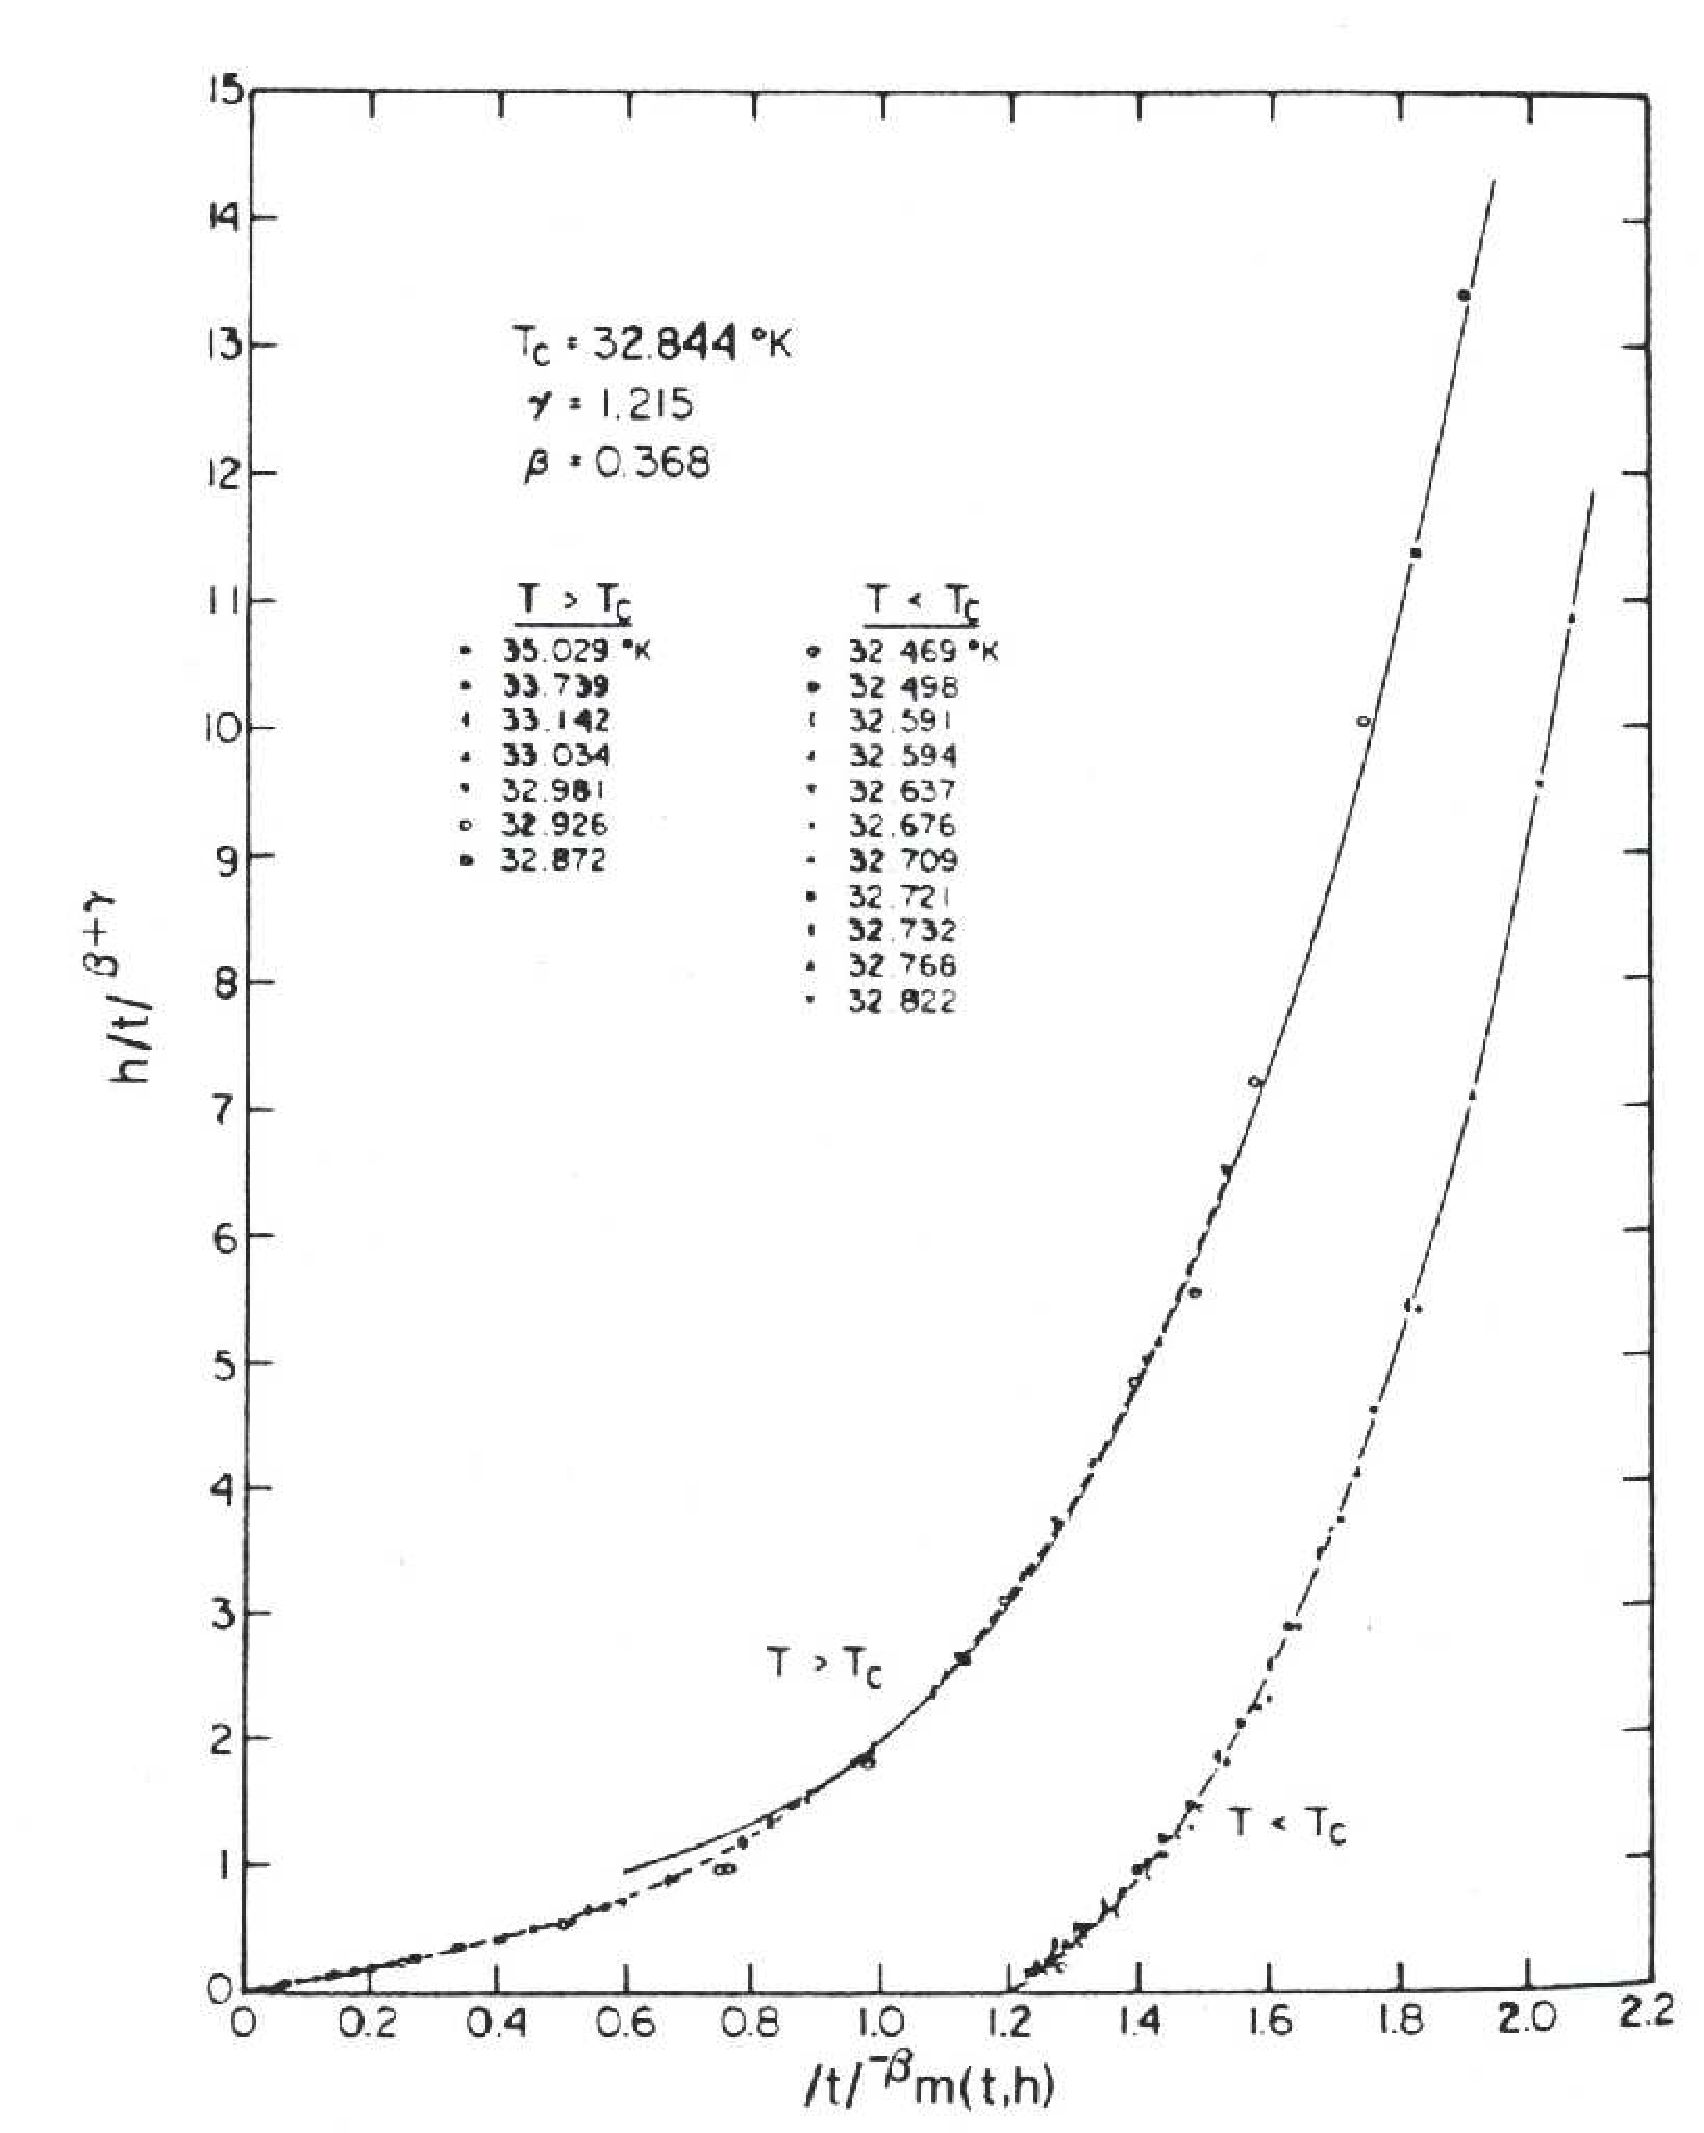
\includegraphics[width=18.0cm,clip=true]{Figs/scaling1}}
%\caption{Magnetisation of CrBr$_3$ in the critical region plotted in scaled form.}
%\end{figure}
%\es
%%%%%%%%%%%%%%%%%%%%%%%%%%%%%%%%%%%%%%%%%%%%%%%%%%%%%%%%%%%%%%%%%%%%

%%%%%%%%%%%%%%%%%%%%%%%%%%%%%%%%%%%%%%%%%%%%%%%%%%%%%%%%%%%%%%%%%%%%%%
\bs
\slidetitle{\small Computer simulation}

\bi

\item Simulation widely used to study critical point phenomena,

\item But computational constraints restict one to dealing with systems of
finite-size.

\item Cannot access the regime of truly long ranged fluctuations that characterize the
near-critical regime. 

\item As a consequence, the critical singularities in
$C_v$, order parameter, etc. appear rounded and shifted in a simulation
study.  

\centerline{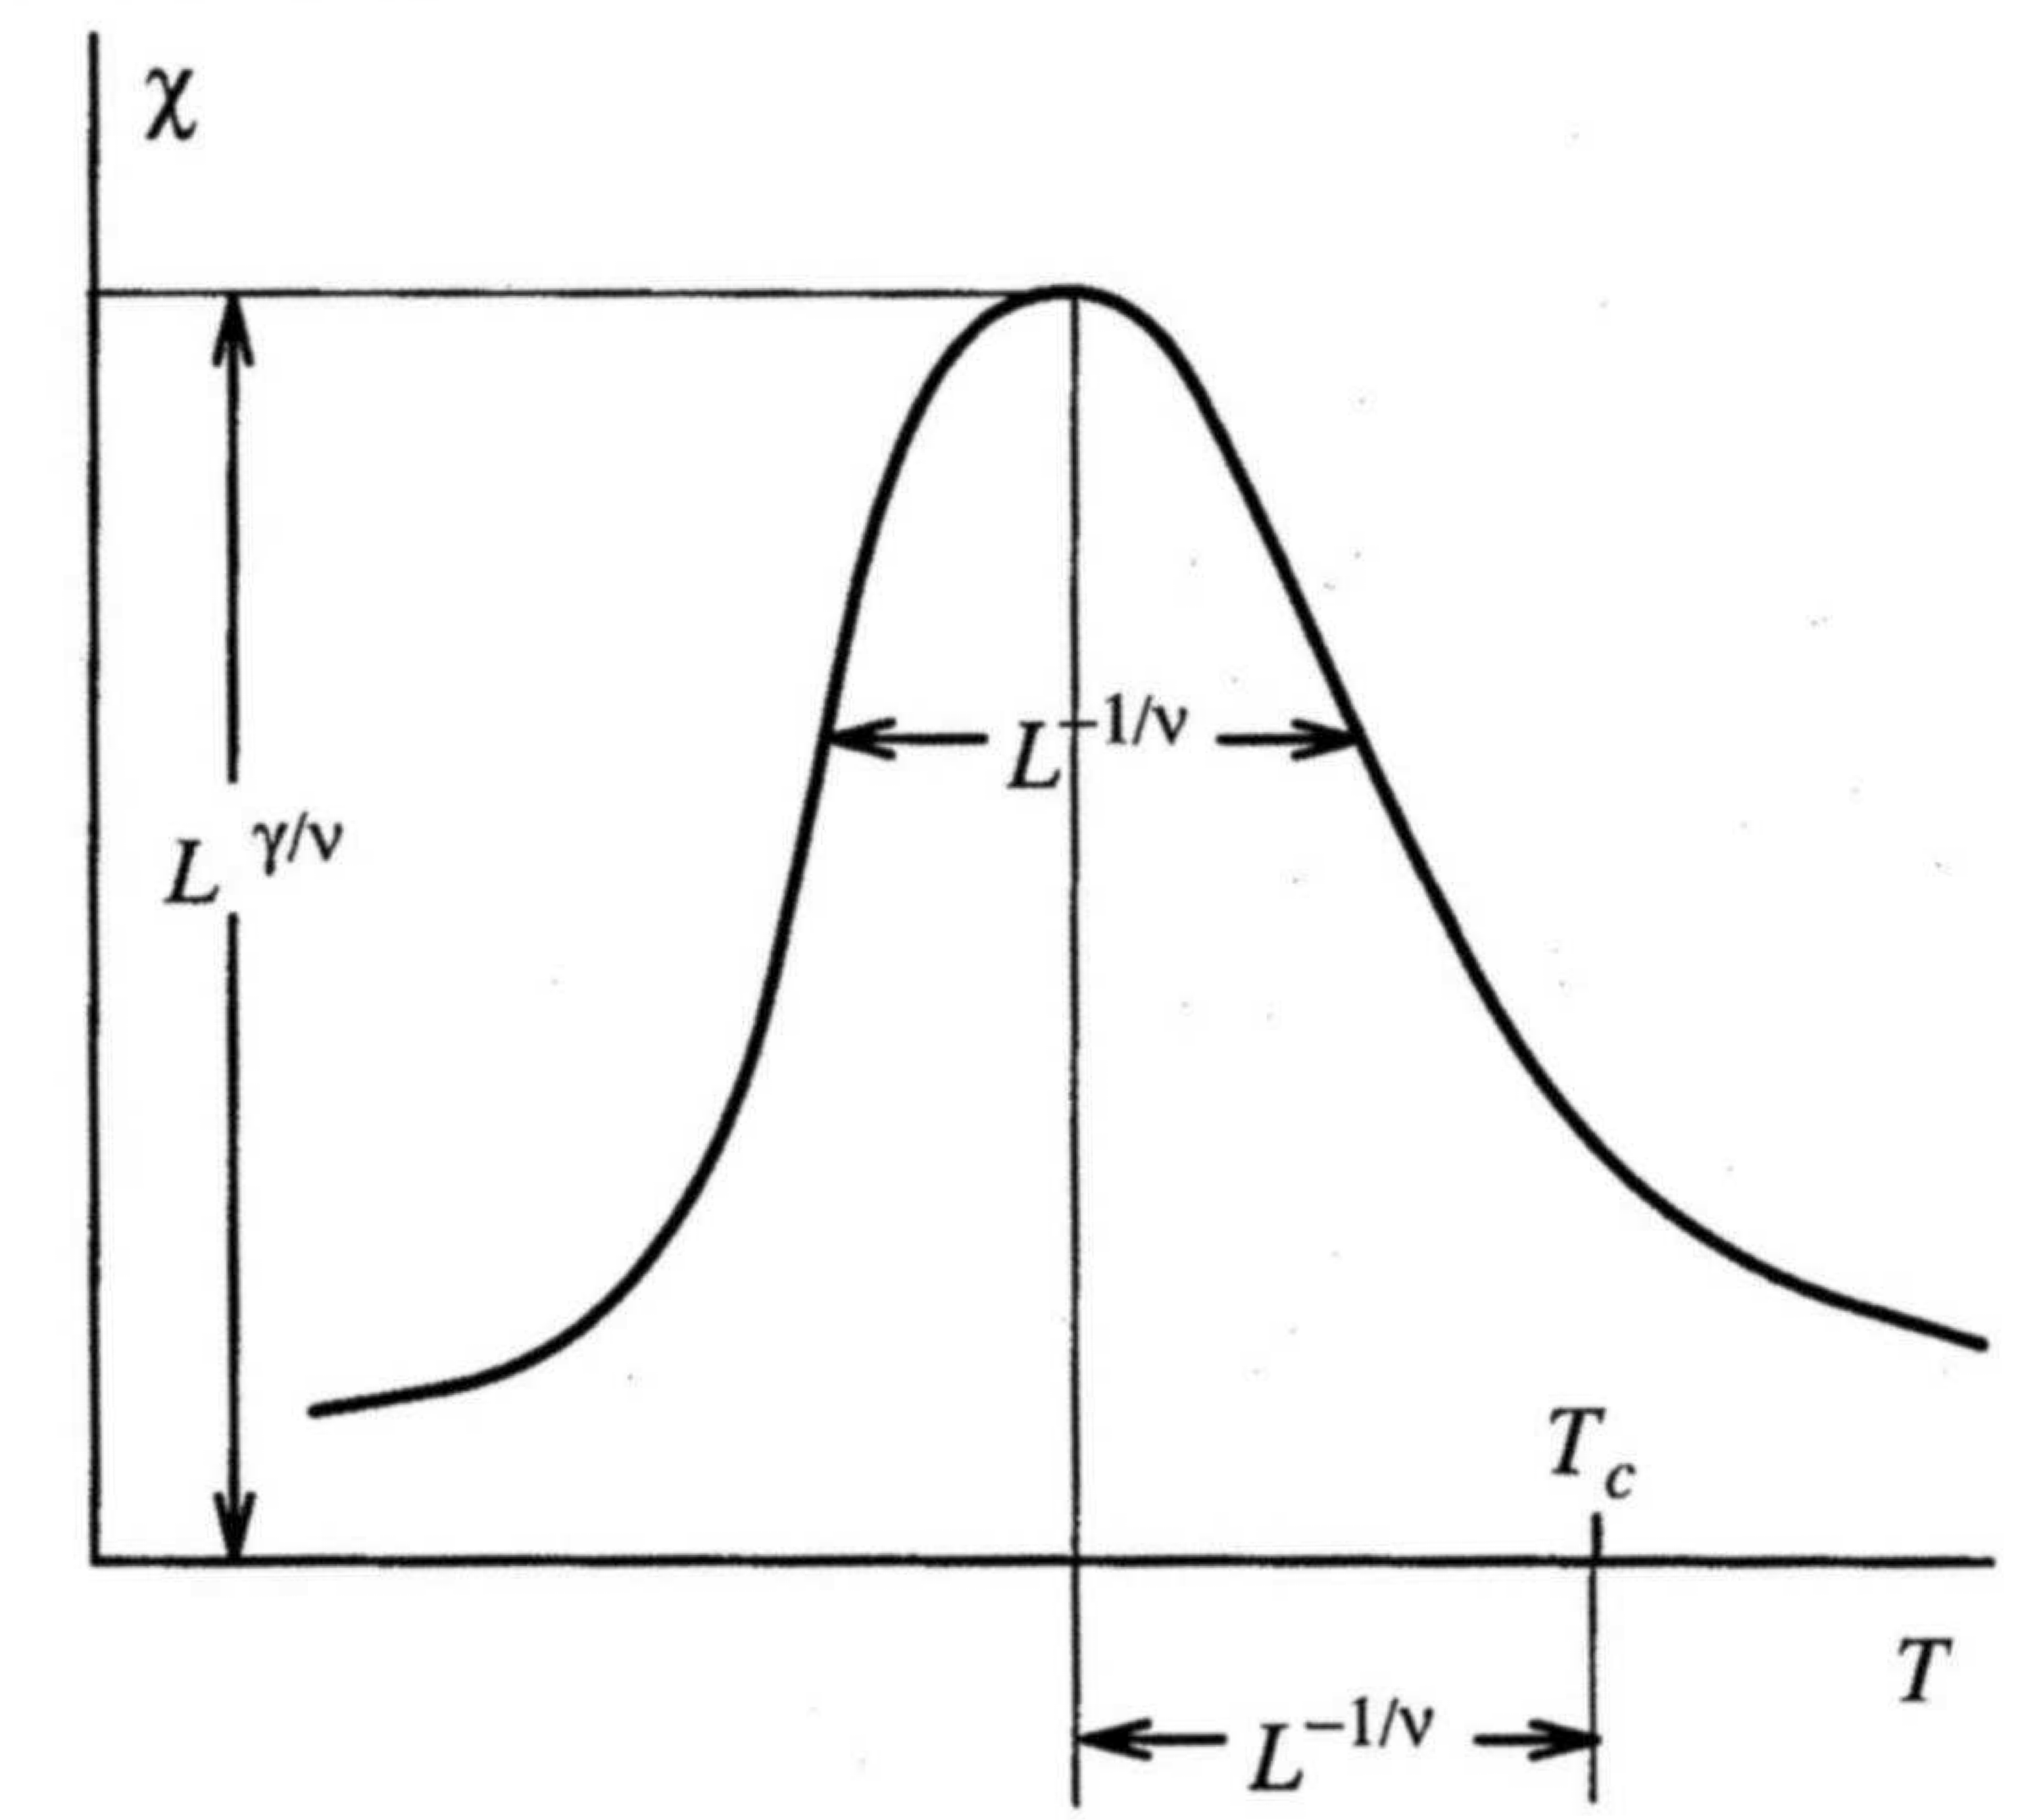
\includegraphics[width=9.3cm,clip=true]{Figs/shift}}

\ei
\es
%%%%%%%%%%%%%%%%%%%%%%%%%%%%%%%%%%%%%%%%%%%%%%%%%%%%%%%%%%%%%%%%%%%%

\bs\bi

\item The peak position does not provide an accurate estimate
of the critical temperature.

\item Although the degree of rounding and shifting
reduces with system size,  it still makes it hard access to the largest system sizes which would
provide accurate estaimates of critical parameters.

\item  To deal with this, finite-size scaling 
methods have been developed.

\item FSS allows extraction of bulk critical properties from simulations
of finite size (see later)

\ei
\es

\bs

\slidetitle{\small Renormalisation Group Theory}

\bi

\item Critical region is characterised by  correlated microstructure on
$\underline{all}$ length-scales up to and including the correlation
length. 

\item Can only be accurately characterised by a very large number of
variables. 

\item MFT and series expansion fail because they at best
incorporate interactions among only a few nearby spins.

\item The scaling hypothesis fails to provide more than qualitative
insight because it focuses on only one length-scale, effectively $\xi$.

\item To obtain a fuller understanding of the critical region, 
must take account of existence of structure on all length-scales. 

\ei
\es
%%%%%%%%%%%%%%%%%%%%%%%%%%%%%%%%%%%%%%%%%%%%%%%%%%%%%%%%%%%%%%%%%%%%%

\bs

\slidetitle{\small The critical point: A many length scale problem}

\bi
\item A near critical system can be characterised by three important length
scales, namely

\begin{enumerate}

\item[(a)] The correlation length, $\xi$, ie the size of correlated
microstructure.

\item[(b)] Minimum length scale $L_{\rm min}$, i.e. the smallest length in
the microscopics of the problem, e.g. lattice spacing of a magnet or the
particle size in a fluid.

\item[(c)] Macroscopic size $L_{max}$ eg. size of the system.

\end{enumerate} 

The authentic critical region is defined by a window condition:

\[
L_{\rm max} \gg \xi \gg L_{\rm min}
\]

\item This regime is hard to tackle because it is characterised by
configurational structure on all scales between $L_{\rm min}$ and $\xi$
(it is fractal). Moreover structure on different length scales are
correlated with one another.

\ei
\es
%%%%%%%%%%%%%%%%%%%%%%%%%%%%%%%%%%%%%%%%%%%%%%%%%%%%%%%%%%%%%%%%%%%%

\bs 
\slidetitle{\small Philosophy and Methodology of the RG} 
\bi 

\item {\bf Central idea}: a stepwise elimination of the degrees of freedom of
the system on successively larger length-scales. 

\item Introduce a fourth length scale $L$, which in contrast to the
other three, characterises the {\em description} of the system.

\item $L$ typifies the size of the smallest resolvable detail in a
description of the system's microstructure.

\item Ising model snapshots contain {\em all}
details of each configuration: the resolution length $L$ in
coincides with the lattice spacing i.e. $L=L_{\min}$.

\item But explicit form of the small scale microstructure is
irrelevant to the behaviour of $\xi$. The small scale microstructure is
 'noise'.

\item To eliminate it, select a larger value of $L$, the resolution
(or `coarse-graining') length

\ei
\es

%%%%%%%%%%%%%%%%%%%%%%%%%%%%%%%%%%%%%%%%%%%%%%%%%%%%%%%%%%%%%%%%%%%%
\bs
\bi

\item There are many ways of implementing this coarse-graining procedure.


\item Adopt a simple strategy in which we divide our sample into blocks of
side $L$, each of which contains $L^d$ sites.

\item The centres of the blocks define a lattice of points
indexed by $I=1,2,....,N/L^d$. We associate with each block lattice
point centre, $I$, a coarse-grained or block variable $S_I(L)$ defined
as the spatial average of the local variables it contains:

\[
S_I(L)=L^{-d}\sum_i^Is_i
\]

\item The set of coarse grained coordinates $\{S(L)\}$ are the basic
ingredients of a picture of the system having spatial resolution of
order $L$.

\ei\es
%%%%%%%%%%%%%%%%%%%%%%%%%%%%%%%%%%%%%%%%%%%%%%%%%%%%%%%%%%%%%%%%%%%

\bs
\bi

\item  Coarse graining operation is easily implemented on a computer. 

\item But while the underlying Ising spins can only take
two possible values, the block variables $S_I(L)$ have $L^d+1$ possible
values.

\item Thus, need a more elaborate colour convention to represent block spins.
Adopt a grey scale.

\item Consider the results of coarse-graining configurations typical of three different
temperatures: $T>T_c$, $T<T_c$ and $T=T_c$.

\ei\es
%%%%%%%%%%%%%%%%%%%%%%%%%%%%%%%%%%%%%%%%%%%%%%%%%%%%%%%%%%%%%%%%%%%
\bs

\centerline{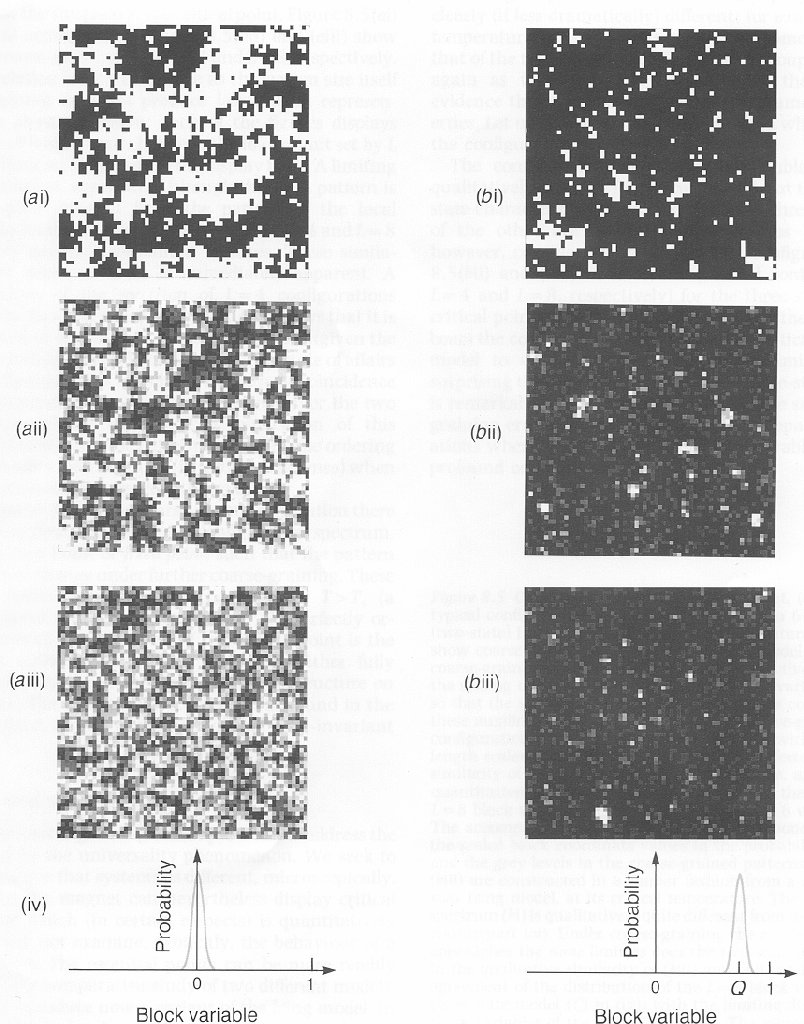
\includegraphics[width=17.5cm,clip=true]{Figs/coarseconf1}}

\es
%%%%%%%%%%%%%%%%%%%%%%%%%%%%%%%%%%%%%%%%%%%%%%%%%%%%%%%%%%%%%%%%%%%

\bs
\bi

\item Two auxiliary operations are implicit in these results. 

\begin{enumerate}

\item First is a {\em length scaling}: the lattice spacing on each
blocked lattice is scaled to that of the original lattice. Can
display correspondingly larger portions of the physical system.

\item Second is a {\em variable scaling}: adjust the scale (`contrast')
of the block variable so as to match block variable spectrum
the full range of grey shades.

\end{enumerate}

\item Consider first a system marginally above $T_c$, having
$\xi\approx 6$. Apply coarse graining with block sizes $L=4$ and
$L=8$.

\item Find that the coarse-graining {\em amplifies}
the consequences of the small deviation of $T$ from $T_c$.

\item As $L$ is increased, the ratio of the size
of the largest configurational features ($\xi$) to the size of the smallest
($L$) is reduced. $\xi/L$ provides a natural measure of how
`critical' is a configuration. 

\ei\es

%%%%%%%%%%%%%%%%%%%%%%%%%%%%%%%%%%%%%%%%%%%%%%%%%%%%%%%%%%%%%%%%%%%
\bs
\bi


\item Thus coarse-graining generates a representation of the system
that is effectively less critical the larger the $L$ value. 

\item Limit is an effectively fully
disordered arrangement. 

\item When viewed on lengthscales $L$ larger than
$\xi$, the correlated microstructure is no longerapparent; each
coarse-grained variable is independent.

\item A similar trend is apparent for $T<T_c$.

\item Again, take $\xi\approx 6$. Coarse-graining with $L=4$ and $L=8$ again generates representations which are
effectively less critical .

\item This time the coarse-graining smoothes out the microstructure
which makes the order incomplete. 

\item The limit point of this procedure is a homogeneously ordered
arrangement.

\ei
\es

%%%%%%%%%%%%%%%%%%%%%%%%%%%%%%%%%%%%%%%%%%%%%%%%%%%%%%%%%%%%%%%%%%%

\bs
\bi

\item Consider now the situation {\em at} the critical point.

\item Since $\xi$ is as large as the system itself,
coarse graining does not produce less critical representations.

\item  In each figure, one sees structure over {\em all} length
scales between the lower limit set by $L$ and the upper limit set by
the display size.

\item A limiting trend is nevertheless apparent. 

\item Although the $L=4$ pattern differs qualitatively from $L=L_{\rm min}$,
the $L=4$ and $L=8$ patterns display qualitatively similar features. 

\item  A statistical analysis of the spectrum of $L=4$ configurations
show that it is almost identical to that of the $L=8$ configurations.

\item Thus patterns formed by the ordering variable at criticality look
statistically the same when viewed on all sufficiently large length scales
(fractal like).

\ei
\es

%%%%%%%%%%%%%%%%%%%%%%%%%%%%%%%%%%%%%%%%%%%%%%%%%%%%%%%%%%%%%%%%%%%%%%%%%%%%%%
\bs
\centerline{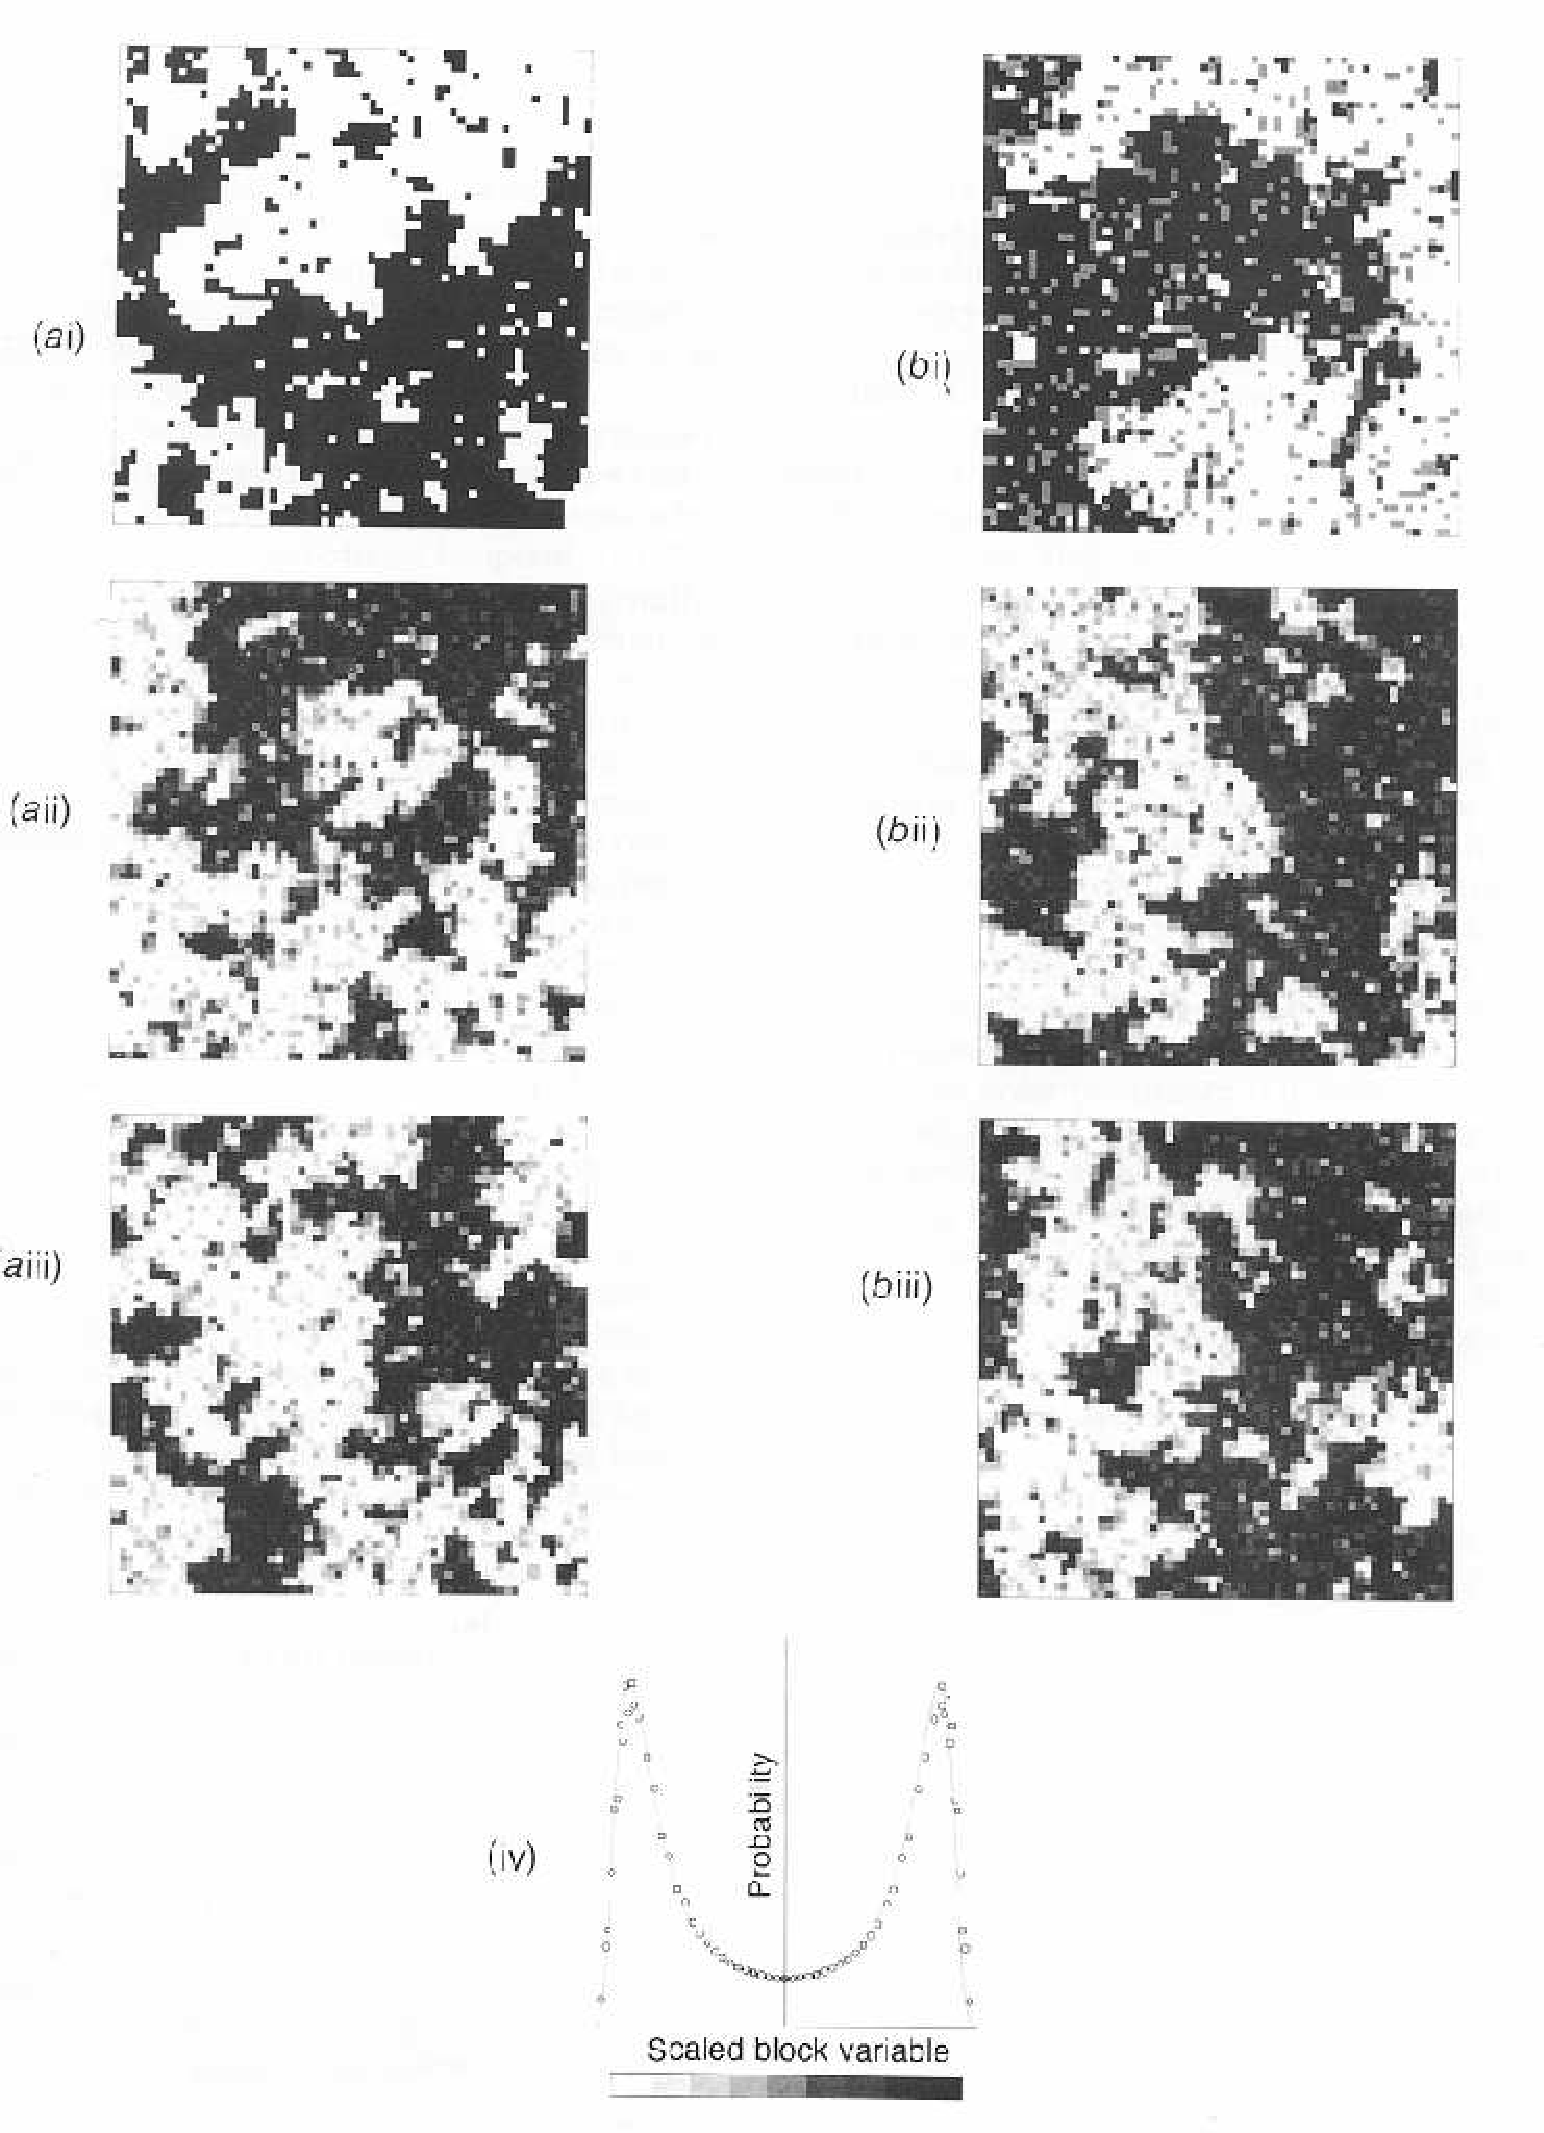
\includegraphics[width=15.0cm,clip=true]{Figs/coarseconf2}}
\es

%%%%%%%%%%%%%%%%%%%%%%%%%%%%%%%%%%%%%%%%%%%%%%%%%%%%%%%%%%%%%%%%%%%%%%%%%%%%%%

\bs
\bi

\item Summary: Under the coarse-graining operation there is an
evolution or {\em flow} of the system's configuration spectrum. 

\item The flow tends
to a limit, or fixed point, such that the pattern spectrum does not
change under further coarse-graining.


\item  These scale-invariant limits have a trivial character for
$T>T_c$, (a perfectly disordered arrangement) and $T < T_c$, (a
perfectly ordered arrangement). 


\item The hallmark of the critical point is the existence of a
scale-invariant limit which is neither fully ordered nor fully
disordered but which possesses structure on all length scales. 

\ei\es


%%%%%%%%%%%%%%%%%%%%%%%%%%%%%%%%%%%%%%%%%%%%%%%%%%%%%%%%%%%%%%%%%%%%%%%%%%%%%%

\bs

\slidetitle{\small Universality and scaling}

\bi

\item Introduce a three state (spin-1) variant of the Ising model.
($s_i=1, 0, -1$).

\item 2-state and 3-state model have properties which are clearly
different: eg. $T_c$ for the 3-state model is some $30\%$
lower than that of the 2-state model.

\item However, the two models  have the same
universal properties. Let us explore the differences and similarities
in the configurations.

\item Raw spin configurations are different.

\item As with 2-state model, coarse-graining operation bears the
configuration spectrum to a non-trivial scale-invariant limit.

\item Remarkably, the limit is the same for both models! Coarse-graining
erases the local differences apparent in configs, and exposes a profound configurational
similarity.

\ei\es

%%%%%%%%%%%%%%%%%%%%%%%%%%%%%%%%%%%%%%%%%%%%%%%%%%%%%%%%%%%%%%%%%%%%%%%

\bs
\bi

\item Similarity of the configurations of the different systems is not
restricted to $T_c$ itself.

\item Suppose we have a 2-state model and a 3-state model each as some 
$t>0$. 

\item Systems will have different correlation lengths,
$\xi_1=a_1t^{-\nu}$ and $\xi_2=a_2t^{-\nu}$.


\item Although this difference survives the coarse-graining itself, it
can be suppressed by the combined coarse graining and
the auxiliary {\em length-scale} operations.

\item Specifically, we choose lengths $L_1$ for $L_2$ for the
two models such that $\xi_1/L_1=\xi_2/L_2$. 

\item We adjust the snapshot sizes so that the sizes of the
minimum-length-scale structure (set by $L_1$ and $L_2$) looks the same
for each system

\item Then the configurations again
look (statistically) identical. Precisely what they look like depends
upon our choice if $\xi/L$.

\ei
\es

%%%%%%%%%%%%%%%%%%%%%%%%%%%%%%%%%%%%%%%%%%%%%%%%%%%%%%%%%%%%%%%%%%%%%%%%%
\bs
\slidetitle{\small Fluid-magnet universality}

\bi

\item The similarities in the critical behaviour of fluids and magnets can be
traced to the underlying similarity in their coarse-grained
configurations 

\ei
\vspace*{1cm}
\centerline{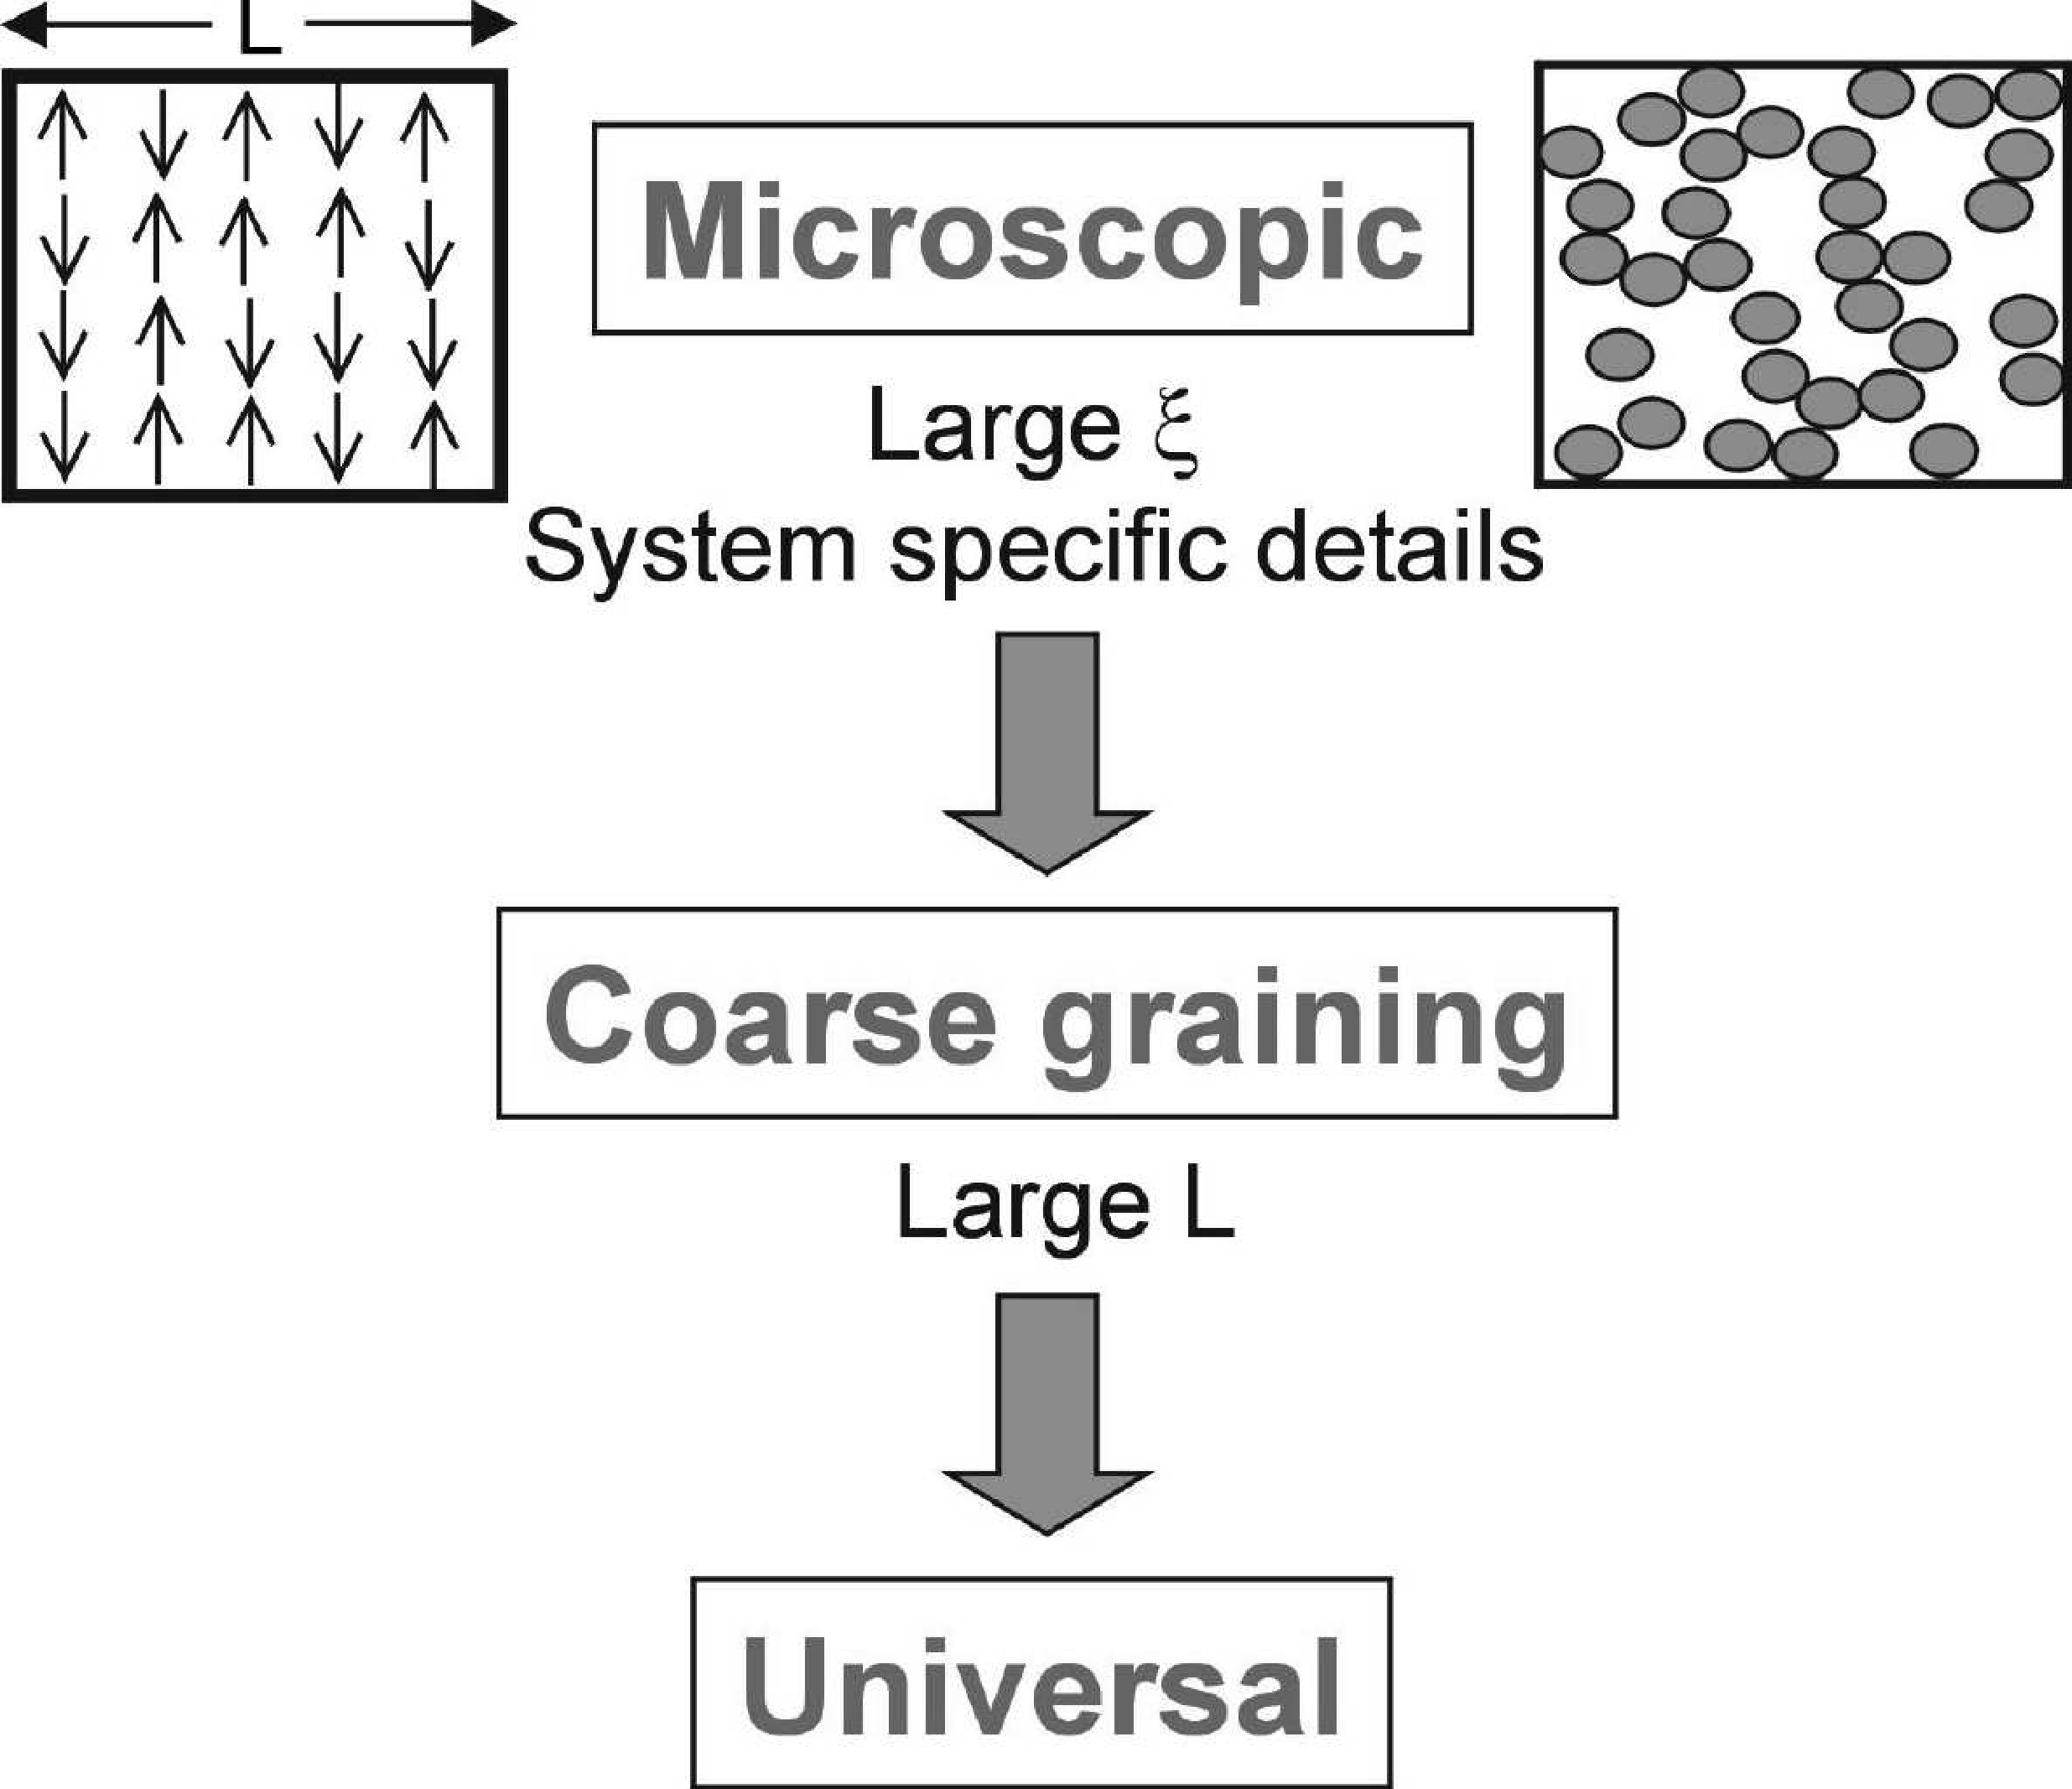
\includegraphics[width=8.3cm,clip=true]{Figs/coarse}}

\bi

\item In a magnet, the relevant configurations are those formed by the
coarse-grained magnetisation (the magnetic moment averaged over a block
of side $L$).

\item In a fluid, the relevant configurations are those of the
coarse-grained density (the mass averaged over a block if side $L$)

\ei\es
%%%%%%%%%%%%%%%%%%%%%%%%%%%%%%%%%%%%%%%%%%%%%%%%%%%%%%%%%%%%%%%%%%%%%%%%%

\bs\bi

\item Patterns of bubbles of liquid or vapour may be matched to
pattern in the former (microdomains of the magnetisation), given
appropriate scaling operations to camouflage the differences between
the length scales and the differences between the variable scales

\vspace*{2cm}

\centerline{\includegraphics[width=8.3cm,clip=true]{Figs/isingconf_new}\hspace*{5mm}\includegraphics[width=8.5cm,clip=true]{Figs/ljconf}}

\ei
\es

%%%%%%%%%%%%%%%%%%%%%%%%%%%%%%%%%%%%%%%%%%%%%%%%%%%%%%%%%%%%%%%%%%%%%%%%%

\bs
\slidetitle{\small Universality classes}
\bi

\item Coarse graining does not erase all differences between the physical
properties of critical systems. 


\item Differences in the space dimension $d$
of two critical systems will lead to different universal properties
such as critical exponents. 

\item Eg. critical exponents of the 2D magnet, match those of the 2d
fluid, but they are different to those of 3d magnets and fluids. 

\ei

{\tiny
%\begin{table}[h]
\begin{center}
\begin{tabular}{|c|c|c|}\hline
$\:$ &  $d=2$ & $d=3$ \\ \hline
{\rm Critical temperature} & $0.5673$ & $0.75$ \\
{\rm Order parameter exponent} $\beta$ & $\frac{1}{8}$ &
$0.325 \pm 0.001$ \\
{\rm Susceptibility exponent} $\gamma$ &  $\frac{7}{4}$ & $1.24 \pm 0.001$ \\
{\rm Correlation length exponent} $\nu$ &  $1$ &
$0.63\pm 0.001$ \\ \hline
\end{tabular}
\end{center}
%\end{table}
}

\bi
\item $d$ is one of a small set of qualitative features which survive
coarse graining and which together serve to define the system's
universal behaviour, or {\em universality class}.
\ei
\es
%%%%%%%%%%%%%%%%%%%%%%%%%%%%%%%%%%%%%%%%%%%%%%%%%%%%%%%%%%%%%%%%%%%%%%%%%%

\bs

\bi

\item Set includes the number of components $n$ of the order
parameter. For the fluid and magnet the order parameter is a scalar,
for which $n=1$. 

\item In some ferromagnets, the order parameter may be a vector ($n=2$
or $n=3$).

\item A third important feature which can change the universality class of a
critical system is the range of the interaction potential between its
constituent particles. 

\item For the Ising model, interactions are inherently nearest
neighbour in range. 

\item Most fluids interact via short ranged dispersion forces.

\item However some systems (such as charged systems) have much longer
ranged interactions and thus different critical exponents to the Ising
model and fluid.

\ei \es
%%%%%%%%%%%%%%%%%%%%%%%%%%%%%%%%%%%%%%%%%%%%%%%%%%%%%%%%%%%%%%%%%%%%%%%%

\bs
\slidetitle{\small Critical exponents}

\bi
\item How can the critical exponents, be computed from the properties of the
coarse-grained configuration spectrum?

\item Consider one typical coarse-grained variable of our Ising system,
which we shall denote $S(L)$. 

\item Suppose that $t$ is sufficiently small that the important
observables are dominated by large-scale microstructure: $\xi \gg
L_{\rm min}$.

\item Configurational universality is expressed in the claim that, for
  {\em any} $L$ and $t$, scale factors $a(L)$ and $b(L)$ may be found
  such that the probability distribution $p(S(L))$ of the
  coarse-grained variable can be written in the form

\[
p(S(L),t)=b(L)\tilde{p}(b(L)S(L),a(L)t)
\]
where $\tilde{p}$ is a function unique to a universality class.

\ei
\es
%%%%%%%%%%%%%%%%%%%%%%%%%%%%%%%%%%%%%%%%%%%%%%%%%%%%%%%%%%%%%%%%%%%%%%

\bs
\bi

\item The role of the scale factors $a$ and $b$ is to absorb the basic
non-universal scales identified before. 

\item Values of exponents are implicit in the $L$ dependence of these
scale factors. The key results are
\vspace*{-1cm}

\begin{eqnarray*}
a(L)&=&a_0L^{1/\nu}\nonumber \\
b(L)&=&b_0L^{\beta/\nu}
\end{eqnarray*}
The amplitudes $a_0$ and $b_0$ are system specific (non-universal)
constants.

\item Thus the basic critical exponents ($1/\nu$, $\beta/\nu$) serve to
characterise the ways in which the configuration spectrum evolves under
coarse-graining. 


\ei
\es
%%%%%%%%%%%%%%%%%%%%%%%%%%%%%%%%%%%%%%%%%%%%%%%%%%%%%%%%%%%%%%%%%%%%%%%

\bs
\bi
\item Consider first $\beta/L$. 

\item Precisely at criticality, the overall scale of the coarse-grained
variable $S(L)$ is eroded with increasing $L$. 

\item Need to amplify scale of $S(L)$ to match configurations of
coarse-graining length $L_1$ to those of a larger length
$L_2$.

\item Required amplification is $b(L_2)/b(L_1)=(L_2/L_1)^{\beta/\nu}$.

\item The index $\beta/\nu$ thus controls the rate at which the scale of the
ordering variable decays with increasing coarse-graining length.
\ei
\es

%%%%%%%%%%%%%%%%%%%%%%%%%%%%%%%%%%%%%%%%%%%%%%%%%%%%%%%%%%%%%%%%%%%%%%%%

\bs
\bi

\item  Consider now $1/\nu$. 

\item For small but finite $t$ (large but finite $\xi$) there is second
way in which the configuration spectrum evolves with $L$. 

\item As noted previously, coarse graining reduces the ratio of $\xi$
to $L$, and results in configurations with a less critical appearence. 

\item More precisely, increasing $L$ from $L_1$ to $L_2$ at constant
$t$ has the same effect as keeping $L$ constant while amplifying the
reduced temperature $t$ by a factor $a(L_2)/a(L_1)=(L_2/L_1)^{1/\nu}$.

\item  One may think of the combination $a(L)t$ as a measure of the effective reduced
temperature of the physical system viewed with resolution length $L$.

\ei
\es

%%%%%%%%%%%%%%%%%%%%%%%%%%%%%%%%%%%%%%%%%%%%%%%%%%%%%%%%%%%%%%%%%%%%%%

\bs
\slidetitle{\small Finite-size scaling}

\bi

\item Consider the average of the block variable $S(L)$. 

\item This is  non other than the value of the
order parameter $Q$, measured over a block of side $L$.

\item Now the block variable average $\bar {S}(L)$ is defined by the first moment of
the probability distribution $p$, i.e.

\[
Q(L,t)=\bar {S}(L,t)=\int S(L)p(S(L),t)dS(L)
\]

substituting for $p(S(L),t)$ gives
{\small
\begin{eqnarray*}
Q(L,t) &=& \int S(L)b(L)\tilde{p}(S(L)b(L),a(L)t)dS(L)\nonumber \\
       &=& b^{-1}(L)\int S(L)b(L)\tilde{p}(S(L)b(L),a(L)t)d(S(L)b(L))\nonumber\\
       &=& b^{-1}(L)f(a(L)t)\nonumber\\
       &=& b_0L^{-\beta/\nu}f(a_0L^{1/\nu}t)
\end{eqnarray*}
}
where $f$ is a universal function (defined by the first moment of $\tilde{p}$).

\ei
\es
%%%%%%%%%%%%%%%%%%%%%%%%%%%%%%%%%%%%%%%%%%%%%%%%%%%%%%%%%%%%%%%%%%%%%%%%%%

\bs
\bi

\item FSS provides us with a prescription for measuring critical
exponent ratios $\beta/\nu$ and $1/\nu$ via computer simulations of
near critical systems.

\item For instance, at criticality ($t=0$) and for finite $L$
$Q(L,0)$ will not be zero (the $T$ at which $Q$ vanishes for finite $L$
is above  the true $T_c$). 

\item However, we know that its value must vanish
in the limit of infinite $L$;  it does so like

\[
Q(L,0)=b_0L^{-\beta/\nu}f(0)\equiv Q_0L^{-\beta/\nu}
\]

\item Thus by studying the critical point $L$ dependence of $Q$ we can 
estimate $\beta/\nu$. 

\item A similar approach in which we study two block
sizes $L$, and tune $t$ separately in each case so that the results 
for $QL^{\beta/\nu}$ are identical provides information on the value of
$1/\nu$.

\ei
\es
%%%%%%%%%%%%%%%%%%%%%%%%%%%%%%%%%%%%%%%%%%%%%%%%%%%%%%%%%%%%%%%%

\bs
\slidetitle{\small The renormalisation group: effective coupling viewpoint}

\bi

\item Return to our fundamental equation 

\[
p = Z^{-1}e^{-\ham}
\]
where $\ham\equiv E/k_BT$.

\item Imagine that we generate, via simulation procedure, a sequence of configurations with
relative probability $\exp(-\ham)$. 

\item Use these to produce a set of coarse-grained configurations. 

\item Q: What is the energy function $\ham^\prime$ of the
coarse-grained variables which would produce these coarse-grained
configurations with the correct relative probability
$\exp(-\ham^\prime)$? 

\ei
\es
%%%%%%%%%%%%%%%%%%%%%%%%%%%%%%%%%%%%%%%%%%%%%%%%%%%%%%%%%%%%%%

\bs
\bi
\item Clearly the form of $\ham^\prime$ depends on the form of $\ham$, thus

\[
\ham^\prime=R(\ham)
\]

\item The operation $R$, defines the RG transformation linking the
coarse-grained configurational energy to the microscopic Hamiltonian.

\item Suppose our system is near criticality and that we wish to calculate
its large-distance properties. 

\item Structure on all length-scales renders basic Stat Mech problem difficult.

\item Make it easier by tackling the not-quite-so-many-length-scale
problem, described by the energy $\ham^\prime$.

\item Large-distance properties of this coarse-grained system are
the same as the large-distance properties of the physical system.

\item Stat. Mech. of $\ham^\prime$ poses a  a problem which is easier (less critical).

\ei
\es

%%%%%%%%%%%%%%%%%%%%%%%%%%%%%%%%%%%%%%%%%%%%%%%%%%%%%%%%%%%%%%%%%%%

\bs
\bi

\item The benefits accruing from this procedure may be amplified by
repeating it.

\item Repeated application of the RGT will eventually result in a
coarse-grained $\ham$ describing configurations in which $\xi$ is no
bigger than the minimum length scale. 

\item The associated coarse-grained system is far from criticality. Its
properties may be reliably computed by mean field or series expansion
methods.


\item These properties are the desired large-distance properties of the
physical system. 

\ei
\es

%%%%%%%%%%%%%%%%%%%%%%%%%%%%%%%%%%%%%%%%%%%%%%%%%%%%%%%%%%%%%%%%%%

\bs
\bi

\item Let us return to the Ising model.

\item Generalise it to include other kinds of interactions. eg.
products of 2nd neighbour spins with strength $J_2$ or, 3rd
nearest neighbours with strength $J_3$.

\item Can allow a family of exchange couplings $J_1$,$J_2$,$J_3,\dots$,
or $J_a, a = 1,2,\dots$ In reduced units, the equivalent coupling
strengths are $K_a =J_a/k_BT$. Their values determine uniquely the
energy for any given configuration.

\item Under the coarse-graining procedure,  $\ham^\prime$ will
be expressible in terms of some new coupling strengths $K^\prime$
describing the interactions amongst the block spin variables 

\item The RGT states that $K_1^\prime$ is some function $f_1$ of all the
original couplings:

\[
K^\prime_a=f_a(K_1,K_2,\dots) =f_a({\bf K}),\hspace*{2mm} a= 1, 2,\dots
\]
where ${\bf K}=K_1, K_2,\dots$

\ei
\es
%%%%%%%%%%%%%%%%%%%%%%%%%%%%%%%%%%%%%%%%%%%%%%%%%%%%%%%%%%%%%%%%%%%

\bs\bi

\item NB It necessary to allow for other types of interactions because
even if we start with only the nearest neighbour coupling in $\ham$ the
transformation will in general produce others in $\ham^\prime$. 

\ei
\es
%%%%%%%%%%%%%%%%%%%%%%%%%%%%%%%%%%%%%%%%%%%%%%%%%%%%%%%%%%%%%%%

\bs

\slidetitle{Example}

\vspace*{2cm}
%\begin{figure}[h]
\centerline{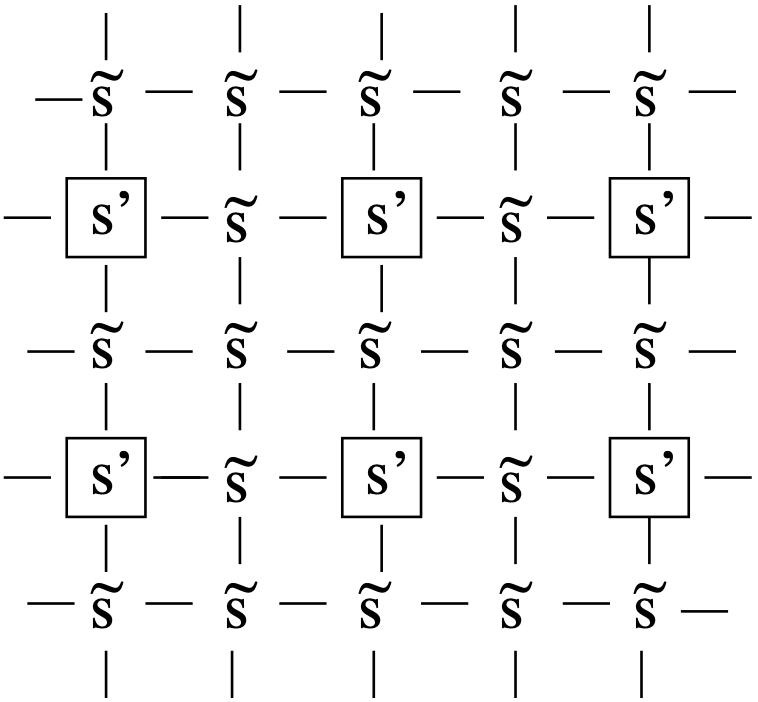
\includegraphics[width=6.3cm,clip=true]{../Figs/rglat}}
%\end{figure}

\bi

\item Consider a simple 2D Ising model.

\item Simple coarse graining scheme -- `decimation': Divide spins into two sets:  $\{s^\prime\}$ form a square
lattice of spacing $2$, others denoted by $\{\tilde{s}\}$.

\item Define an effective energy function ${\cal H^\prime}$ for the
$s^\prime$ spins by averaging over all  possible
arrangements of $\tilde{s}$ spins

\[
\exp(-\ham^\prime)=\sum_{\{\tilde {s}\}} \exp(-\ham).
\]

\ei\es

%%%%%%%%%%%%%%%%%%%%%%%%%%%%%%%%%%%%%%%%%%%%%%%%%%%%%%%%%%%%%%%%%%%%%

\bs
\bi

\item The new energy function realizes two basic aims of the
renormalisation group method: 

\bi

\item Long-distance physics still contained in system described by
$\ham^\prime$ (partition functions are the same)

\item New system is `further' from criticality because the ratio of correlation
length to lattice spacing has been reduced by $1/2$  

\ei

\item But how to perform the partial configuration sum?

\item This cannot in general be done exactly (except in 1D--see problem
set 2).

\ei\es
%%%%%%%%%%%%%%%%%%%%%%%%%%%%%%%%%%%%%%%%%%%%%%%%%%%%%%%%%%%%%%%%%%%%%
\bs
\bi

\item Resort to approximations, eg high temperature expansion:

\[
\exp(-{\cal H}/k_BT)=1-{\cal H}/k_BT +\frac{1}{2!}({\cal H}/k_BT)^2+.....
\]


\item Substitute this into RHS of RG transformation
and look for terms which depend on the $s^\prime$ spins after partial summation.

\item Find (see notes) 

\[
K^\prime=K^2   \hspace*{2cm}{\dagger}
\]

\item Many other terms and couplings are generated by the higher orders
of the high temperature expansion. 

\item Need to include these to produce reliable values for the $T_c$
and exponents. 

\ei\es
%%%%%%%%%%%%%%%%%%%%%%%%%%%%%%%%%%%%%%%%%%%%%%%%%%%%%%%%%%%%%%%%%%%%%
\bs\bi

\item But qualitative picture already emerges from above

\item First point is that eq.$\dagger$ has the unstable fixed point $K^*=
1$: the flow of couplings under repeated iteration of eq. $\dagger$ is
away from the fixed point,

\vspace*{1cm}

\centerline{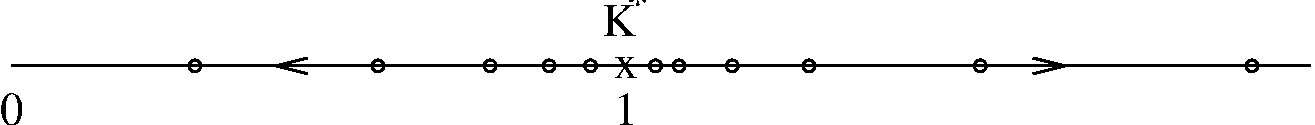
\includegraphics[width=12.3cm,clip=true]{../Figs/flow1}}

\item At criticality, we must identify $K^\prime= K$ since coarse
graining a critical system leaves it critical. Thus $K^*=1$ is
a candidate for the critical point $K_c$,

\[
K_c=J/k_BT_c=1
\]

(In poor agreement with accepted values due to neglect of higher order
terms in series expansion)
\ei\es

%%%%%%%%%%%%%%%%%%%%%%%%%%%%%%%%%%%%%%%%%%%%%%%%%%%%%%%%%%%%%%%%%%%%%
\bs
\bi

\item Can also get information on critical exponents. Expanding eq.~$\dagger$
about $K=K^\star$ we find

\[
K^\prime - K^* = 2 (K - K^*)+ (K - K^*)^2 
\]

\item Close to criticality, can neglect final term.

\item Thus deviation of coupling from its fixed
point (critical) value is bigger for the new system than it is for
the old by a factor of two $\Rightarrow$ reduced temperature is
also bigger by a factor of two:  

\[
t^\prime= 2t     
\]

\item But correlation length is smaller by a factor of $1/2$ (by construction):

\[
\xi^\prime= \xi/2     
\]

Thus, when we double $t$, we halve $\xi$, implying that 

\[
\xi\propto t^{-1}
\]
i.e $\nu=1$.
\ei\es
%%%%%%%%%%%%%%%%%%%%%%%%%%%%%%%%%%%%%%%%%%%%%%%%%%%%%%%%%%%%%%%%%%%%%

\bs
\slidetitle{Universality}

\bi

\item In order to expose universality, should allow for several
different kinds of coupling $J_a$, and show how systems with {\em
different} $J_a$ can have the {\em same} critical behaviour. 


\item Can form a representation of the space of all coupling
strengths $K_a$ in the energy function $\ham/k_BT$.

\centerline{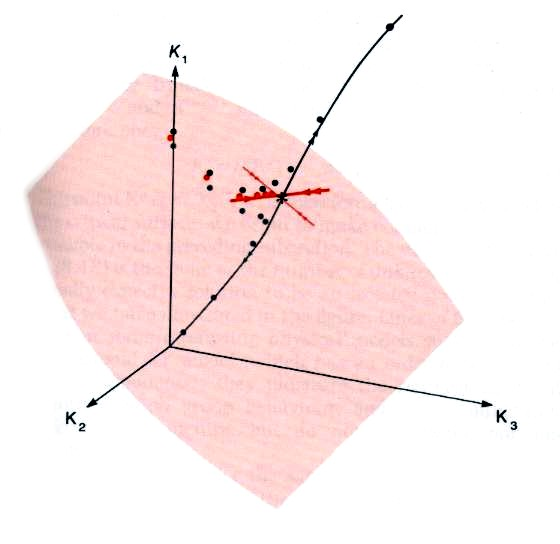
\includegraphics[width=12.3cm,clip=true]{Figs/flow2}}

\ei
\es

%%%%%%%%%%%%%%%%%%%%%%%%%%%%%%%%%%%%%%%%%%%%%%%%%%%%%%%%%%%%%%%%

\bs
\bi

\item Each ``ray'' from the origin represents the temperature behaviour
of a given model. Points on a ray close to the origin represent the
high $T$ behaviour.

\item Points far from the origin represent the low $T$ behaviour. 

\item The critical point is represented by a specific point on this
ray, $K_a= J_a/k_BT, a= 1,2,\dots$ .

\item The set of critical points on all of the
possible rays forms a {\em surface}, the critical surface.


\item Our immediate goal then is to understand how the RGT can explain why
different physical systems near this critical surface have the same
behaviour.


\ei
\es

%%%%%%%%%%%%%%%%%%%%%%%%%%%%%%%%%%%%%%%%%%%%%%%%%%%%%%%%%%%%%%%%%%%%%%
\bs

\bi

\item Suppose we start with a physical system,
with coupling strengths $K_a,  a= 1,2, \dots$. 

\item RGT generate a new point in the figure, at the coupling strengths
$K_a^{(1)}=f_a({\bf K})$; these are the couplings appearing in the
effective energy function describing the coarse-grained system.

\item Repeating the transformation, gives a new $\ham^\prime$ with coupling
strengths $K_a^{(2)}=f_a({\bf K})$. 

Repeated RGTs $\to$ a flow of points in the figure: ${\bf K\to
K^{(1)}\to\dots\to K^{(n)}}$ 

\item Consider the coupling flow for the  Ising model at its critical
point. $L/\xi$ remains infinite after any finite number of steps. 

The behaviour of the coupling flows tends to a limit, $K^*$, i.e.

\[
K^*_a=f_a(K^*)\hspace*{6mm} a= 1,2 .....         
\]

\item This point ${\bf K^*} \equiv K_1^*, K_2^*, \dots$ is therefore a {\em fixed
point} which lies in the critical surface.

\ei\es

%%%%%%%%%%%%%%%%%%%%%%%%%%%%%%%%%%%%%%%%%%%%%%%%%%%%%%%%%%%%%%%%%%%%%%

\bs
\bi

\item Now consider the Ising model  at temperature $T>T_c$;

\item New flow appears initially to
follow towards the same fixed point.

\item However, the flow must eventually move away from the fixed point
because each coarse-graining now produces a model further from
criticality.

\item The resulting flow is represented schematically by one set of black dots
and tends to the high temperature fixed point.

\item Similarly for $T<T_c$, the flow ultimately converges on the low
temeprature fixed point.

\item We are now in a position to understand universality within this framework.

\ei
\es

%%%%%%%%%%%%%%%%%%%%%%%%%%%%%%%%%%%%%%%%%%%%%%%%%%%%%%%%%%%%%%%%%%%%%%
\bs
\bi

\item We will suppose that there exists a single fixed point in the
critical surface which sucks in all flows starting from a point in that
surface.

\item Any system at its critical point will exhibit large-length scale
physics (large-block spin behaviour) described by the single set of
fixed point coupling constants.

\item The uniqueness of this limiting set of coupling constants is the
essence of critical point universality.

\ei
\es
\end{document}



\bs
\slidetitle{Variational approach}
\bi

\item More systematic strategy: choose a trial probability
distribution for the spins $p_0(\{s\})$, corresponding to a trial Hamiltonian ${\cal H}_0$

\[
p_0(\{s\})=\frac{1}{Z_0}e^{-\beta {\cal H}_0(\{s\})}
\]
where $Z_0=e^{-\beta F_0}$. 

\item Can choose any trial Hamiltonian ${\cal H}_0$ at all though
choice should be easier to deal with than the actual Hamiltonian ${\cal
H}$.

\item Trick: choose ${\cal H}_0$ with one or more parameters. Adjust
these to minimize the free energy. {\em Bogoliubov's inequality}:

\[
F<\Phi=F_0+\langle {\cal H}-{\cal H}_0\rangle_0\:,
\]
where ${\cal H}_0$ depends on parameter $H$; ${\cal H}$ is the real hamiltonian;
and $\langle \cdots \rangle_0$ is an average evaluated with respect
to $p_0(\{s\})$.

\ei
\es
%%%%%%%%%%%%%%%%%%%%%%%%%%%%%%%%%%%%%%%%%%%%%%%%%%%%%%%%%%%%%%%%
\bs\bi

\item For a simple Ising model, a suitably simple trial Hamiltonian is 

\[
{\cal H}_0=-H_0\sum_is_i
\]
Here the effect of interactions with other spins is approximated by each spin seeing the
same ``mean field'' $H_0$. 

\item Corresponding free energy $F_0$ is (exercise): 

\begin{eqnarray*}
F_0 &=&-Nk_BT\ln(2\cosh \beta H_0)\\
\Rightarrow m_0 &=& \langle s_i\rangle_0=\tanh (\beta H_0)
\end{eqnarray*}

\item Also need
\begin{eqnarray*}
\langle {\cal H}-{\cal H}_0\rangle_0 &=& \sum_{\{s\}}({\cal H}-{\cal H}_0)p_0(\{s\})\\
                                     &=& \sum_{\{s\}}(-J\sum_{<ij>}s_is_j+ H_0\sum_i s_i)p_0(\{s\})\\
                                     &=& -J\sum_{<ij>}\langle s_i\rangle_0\langle s_j\rangle_0 + H_0\sum_i\langle s_i\rangle_0\\
                                     &=& -JNqm_0^2/2 + NHm_0
\end{eqnarray*}
where $\langle s_is_j\rangle_0=\langle
s_i\rangle_0\langle s_i\rangle_0=m_0^2$, $Nq/2$ bonds on the lattice.

\ei
\es
%%%%%%%%%%%%%%%%%%%%%%%%%%%%%%%%%%%%%%%%%%%%%%%%%%%%%%%%%%%%%%%%%%%%%%%%
\bs
\bi

\item Bogoliubov's inequality, yields

\[
\Phi= -Nk_BT\ln(2\cosh \beta H_0) -JNqm_0^2/2 + NH_0m_0
\]

\item To find the equilibrium mean magnetisation $m$, minimize $\Phi$
with respect to parameter $H$:

\[
\frac{\partial \Phi}{\partial H_0}=0\:, \hspace*{1cm} \Rightarrow H_0=Jz\tanh \beta H_0
\]

\item Substituting back in to $\Phi$  yields the m.f. free
energy:

\[
F_{mf}=-NK_BT\ln(2\cosh \beta Jqm ) + NJqm^2/2 \;,
\]
which can be differentiated to give the same result as found before:

\[
m=\tanh(\beta qJm)
\]

{\bf Exercise}: Show this.

\item Many types of mean field theory can be interpreted in such variational
terms.

\ei
\es

